\documentclass[12pt,oneside]{report}
\usepackage[acronym, nopostdot, nonumberlist]{glossaries}


\makeglossaries
%%%%%%%%%%%%%%%%%%%%%%%%%%%%%%%%%%%%%%%%%%%%%%%%%%%%%%%%%%%%%%%%%%%%%%%%%%%%%

% Definitions for the title page
% Edit these to provide the correct information
% e.g. \newcommand{\reportauthor}{Timothy Kimber}

\newcommand{\reporttitle}{Multi-spectral Image Alignment of Brain Tissue Dissection During Neurosurgery}
\newcommand{\reportauthor}{Muhammad Farhan Oktavian}
\newcommand{\supervisora}{Daniel Elson}
\newcommand{\supervisorb}{Zepeng Hu}
\newcommand{\degreetype}{Medical Robotics and Image-Guided Intervention}

%%%%%%%%%%%%%%%%%%%%%%%%%%%%%%%%%%%%%%%%%%%%%%%%%%%%%%%%%%%%%%%%%%%%%%%%%%%%%

% load some definitions and default packages
%%%%%%%%%%%%%%%%%%%%%%%%%%%%%%%%%%%%%%%%%
% University Assignment Title Page 
% LaTeX Template
% Version 1.0 (27/12/12)
%
% This template has been downloaded from:
% http://www.LaTeXTemplates.com
%
% Original author:
% WikiBooks (http://en.wikibooks.org/wiki/LaTeX/Title_Creation)
%
% License:
% CC BY-NC-SA 3.0 (http://creativecommons.org/licenses/by-nc-sa/3.0/)
% 
%
%%%%%%%%%%%%%%%%%%%%%%%%%%%%%%%%%%%%%%%%%
%----------------------------------------------------------------------------------------
%	PACKAGES AND OTHER DOCUMENT CONFIGURATIONS
%----------------------------------------------------------------------------------------
\usepackage[a4paper,hmargin=2.54cm,vmargin=2.54cm,includeheadfoot]{geometry}
\usepackage{textpos}
\usepackage[sort&compress,numbers]{natbib} % for bibliography
\usepackage{tabularx,longtable,multirow,subfigure,caption}%hangcaption
% \usepackage{fncylab} %formatting of labels
\usepackage{fancyhdr} % page layout
\usepackage{url} % URLs
\usepackage[english]{babel}
\usepackage{amsmath}
\usepackage{graphicx}
\usepackage{dsfont}
\usepackage{epstopdf} % automatically replace .eps with .pdf in graphics
\usepackage{backref} % needed for citations
\usepackage{array}
\usepackage{latexsym}
\usepackage[pdftex,pagebackref,hypertexnames=false,colorlinks]{hyperref} % provide links in pdf

\hypersetup{pdftitle={},
  pdfsubject={}, 
  pdfauthor={},
  pdfkeywords={}, 
  pdfstartview=FitH,
  pdfpagemode={UseOutlines},% None, FullScreen, UseOutlines
  bookmarksnumbered=true, bookmarksopen=true, colorlinks,
    citecolor=black,%
    filecolor=black,%
    linkcolor=black,%
    urlcolor=black}

\usepackage[all]{hypcap}


%\usepackage{color}
%\usepackage[tight,ugly]{units}
%\usepackage{float}
%\usepackage{tcolorbox}
%\usepackage[colorinlistoftodos]{todonotes}
% \usepackage{ntheorem}
% \theoremstyle{break}
% \newtheorem{lemma}{Lemma}
% \newtheorem{theorem}{Theorem}
% \newtheorem{remark}{Remark}
% \newtheorem{definition}{Definition}
% \newtheorem{proof}{Proof}


%%% Default fonts
\renewcommand*{\rmdefault}{bch}
\renewcommand*{\ttdefault}{cmtt}



%%% Default settings (page layout)
\setlength{\parindent}{0em}  % indentation of paragraph

\setlength{\headheight}{14.5pt}
\pagestyle{fancy}
\renewcommand{\chaptermark}[1]{\markboth{\chaptername\ \thechapter.\ #1}{}} 

% \fancyfoot[ER,OL]{\sffamily\textbf{\thepage}}%Page no. in the left on odd pages and on right on even pages
% \fancyfoot[OC,EC]{\sffamily }
% \renewcommand{\headrulewidth}{0.1pt}
% \renewcommand{\footrulewidth}{0.1pt}
% \captionsetup{margin=10pt,font=small,labelfont=bf}


%--- chapter heading

\def\@makechapterhead#1{%
  \vspace*{10\p@}%
  {\parindent \z@ \raggedright \sffamily
    \interlinepenalty\@M
    \Huge\bfseries \thechapter \space\space #1\par\nobreak
    \vskip 30\p@
  }}

%---chapter heading for \chapter*  
\def\@makeschapterhead#1{%
  \vspace*{10\p@}%
  {\parindent \z@ \raggedright
    \sffamily
    \interlinepenalty\@M
    \Huge \bfseries  #1\par\nobreak
    \vskip 30\p@
  }}

\allowdisplaybreaks


%---spacing
\usepackage{setspace}
\onehalfspacing

%---url on bib
\usepackage{url}
\def\UrlBreaks{\do\/\do-}
\usepackage{breakurl}
\usepackage[breaklinks]{hyperref}

%---floaters
\usepackage{float}

% load some macros
% Here, you can define your own macros. Some examples are given below.

\newcommand{\R}[0]{\mathds{R}} % real numbers
\newcommand{\Z}[0]{\mathds{Z}} % integers
\newcommand{\N}[0]{\mathds{N}} % natural numbers
\newcommand{\C}[0]{\mathds{C}} % complex numbers
\renewcommand{\vec}[1]{{\boldsymbol{{#1}}}} % vector
\newcommand{\mat}[1]{{\boldsymbol{{#1}}}} % matrix
\newcommand{\etal}[0]{\textit{et al. }}
\newcommand{\boldit}[1]{\textbf{\textit{#1}}}


\date{September 2023}

\begin{document}

%TC:incbib

% load title page
% Last modification: 2015-08-17 (Marc Deisenroth)
\begin{titlepage}

\newcommand{\HRule}{\rule{\linewidth}{0.5mm}} % Defines a new command for the horizontal lines, change thickness here


%----------------------------------------------------------------------------------------
%	LOGO SECTION
%----------------------------------------------------------------------------------------


\includegraphics[width = 4cm]{./figures/imperial}\\[0.5cm] 

\center % Center remainder of the page

%----------------------------------------------------------------------------------------
%	HEADING SECTIONS
%----------------------------------------------------------------------------------------

\textsc{\Large Imperial College London}\\[0.5cm] 
\textsc{\large Hamlyn Centre}\\[0.5cm] 

%----------------------------------------------------------------------------------------
%	TITLE SECTION
%----------------------------------------------------------------------------------------

\HRule \\[0.4cm]
{ \huge \bfseries \reporttitle}\\ % Title of your document
\HRule \\[1.5cm]
 
%----------------------------------------------------------------------------------------
%	AUTHOR SECTION
%----------------------------------------------------------------------------------------

\begin{minipage}[t]{0.5\textwidth}
\begin{flushleft} \large
\emph{Author:}\\
\reportauthor % Your name
\end{flushleft}
\end{minipage}
~
\begin{minipage}[t]{0.4\textwidth}
\begin{flushright} \large
\emph{Supervisor:} \\
\supervisora \\ % Supervisor's Name 
\supervisorb % Supervisor's Name
\end{flushright}
\end{minipage}\\


%----------------------------------------------------------------------------------------
%	FOOTER & DATE SECTION
%----------------------------------------------------------------------------------------
\vfill % Fill the rest of the page with whitespace
A thesis submitted in partial fulfilment of the requirements\\
for the degree of MRes in \degreetype\\
and for the Diploma of Imperial College\\[0.5cm]

\makeatletter
\@date 
\makeatother


\end{titlepage}



% page numbering etc.
\pagenumbering{roman}
\clearpage{\pagestyle{empty}\cleardoublepage}
\setcounter{page}{1}
\pagestyle{fancy}

%%%%%%%%%%%%%%%%%%%%%%%%%%%%%%%%%%%%
\begin{abstract}Tumour delineation is a difficult part of tumour resection. The tumour margin needs to be defined as best as possible to lower the chance of leaving it behind and taking out healthy tissue. Imperial College London and Charing Cross Hospital have acquired a dataset of multi-spectral images taken during brain surgery. The dataset comprises images from 49 patients, each with several sets of microscope colour images, spectral image stacks and labels. However, only the microscope images from the dataset are labelled. Alignment between the microscope images and spectral image stacks, therefore the label, needs to be done before investigating to correlate spectral values to the labelled tissue. In this project, we proposed a method to align the microscope images and labels to the spectral image stack. The steps of the registration pipeline are stack registration, global registration and finer registration. Following the registration, we took 20 patients as samples for analysis based on the image spectral values. Though the registration performs well, further efforts must be made for the spectral image analysis.

\vspace{1.5cm}
\textbf{Word count:} 10,740
\end{abstract}

% \cleardoublepage
%%%%%%%%%%%%%%%%%%%%%%%%%%%%%%%%%%%%
\section*{Acknowledgments}
\paragraph{}
First and foremost, I would like to express my gratitude to my supervisor, Professor Daniel Elson, who made this work possible. His guidance and feedback have been a tremendous help to me in conducting this project. I would also like to thank my co-supervisor, Zepeng Hu, for always helping me with any problems I faced.

\paragraph{}
Second, I would like to sincerely thank all of the MRes program faculty members who gave us valuable knowledge for our time at Imperial and future endeavours.

\paragraph{}
Third, to my parents and siblings, your support and prayers have led me to the position I am in today. I am very grateful for all the efforts that you have put into my life.

\paragraph{}
Lastly, thank you for all the MRes 2022--2023 cohorts. We went through the year together by supporting each other. I am hoping for the best for all of you!

\clearpage{\pagestyle{empty}\cleardoublepage}

%%%%%%%%%%%%%%%%%%%%%%%%%%%%%%%%%%%%
% Abbreviations

\newacronym{auc}{AUC}{Area Under the ROC Curve}
\newacronym{ccd}{CCD}{Charge-coupled Device}
\newacronym{cnn}{CNN}{Convolutional Neural Network}
\newacronym{dlk}{DLK}{Deformable Lucas-Kanade}
\newacronym{gms}{GMS}{Gradient Magnitude Similarity}
\newacronym{gmsd}{GMSD}{Gradient Magnitude Similarity Deviation}
\newacronym{gmsm}{GMSM}{Gradient Magnitude Similarity Mean}
\newacronym{hsi}{HSI}{Hyper-spectral Imaging}
\newacronym{iou}{IoU}{Intersection over Union}
\newacronym{lctf}{LCTF}{Liquid Crystal Tunable Filter}
\newacronym{ml}{ML}{Machine Learning}
\newacronym{mse}{MSE}{Mean-Square Error}
\newacronym{msi}{MSI}{Multi-spectral Imaging}
\newacronym{nn}{NN}{Neural Network}
\newacronym{pfn}{PFN}{Progressive Finite Newton}
\newacronym{psnr}{PSNR}{Peak Signal-to-Noise Ratio}
\newacronym{rgb}{RGB}{red, green and blue}
\newacronym{roc}{ROC}{Receiver Operating Charateristic}
\newacronym{ssim}{SSIM}{Structural Similarity Index Measure}

\printglossary[type=\acronymtype, title=Abbreviations, toctitle=List of abbreviations, style=super]

\clearpage{\pagestyle{empty}\cleardoublepage}

%%%%%%%%%%%%%%%%%%%%%%%%%%%%%%%%%%%%
%--- table of contents
\fancyhead[RE,LO]{\sffamily {Table of Contents}}
\tableofcontents 


\clearpage{\pagestyle{empty}\cleardoublepage}
\pagenumbering{arabic}
\setcounter{page}{1}
\fancyhead[LE,RO]{\slshape \rightmark}
\fancyhead[LO,RE]{\slshape \leftmark}

%%%%%%%%%%%%%%%%%%%%%%%%%%%%%%%%%%%%
\chapter{Introduction}

\paragraph{}
Brain tumours are tumours that affect the central nervous system and can develop in both children and adults. These tumours can be classified under the microscope based on their biopsy sample characteristics. Nevertheless, some tumours are very hard to distinguish, as they are visually indifferent to their surrounding tissue \cite{collins_brain_2004}. Maximal tumour resection through surgical operation is still one of the main treatments for brain tumours \cite{bush_current_2017}. However, the indifferent visual appearance of a tumour might make it difficult to delineate the margin between the tumour and healthy tissue. It is important to have an optimum resection as we do not want to leave any tumour behind, have a chance for it to recur, or take excessive healthy tissue, which might lower brain function.

\paragraph{}
Nowadays, health professionals employ many imaging techniques to help them produce diagnoses. Most of them are imaging modalities that require specialised and expensive equipment, such as X-ray-based computed tomography (CT) or magnetic resonance imaging (MRI). These modalities are often done in the earlier stages of treatment to reinforce diagnostic hypotheses or locate regions of interest prior to surgery. Due to cost and availability constraints, health professionals may opt to use more common equipment, such as ultrasonography (USG), as their first step in diagnosis.

\paragraph{}
In recent years, researchers have shown that images acquired from the modalities mentioned can be analysed and trained upon to solve classification problems \cite{wang_image_2020}, identifying and differentiating objects from an image. Furthermore, there were also efforts to solve the problem in another way, by using colour images composed of three colour channels \acrfull{rgb}, capturing the scene as seen by the health professionals themselves. In addition to its true-to-vision colour, the system to acquire \acrshort{rgb} images is very accessible as most modern smartphones have a camera that is capable of capturing \acrshort{rgb} images.

\paragraph{}
\acrfull{msi} is an imaging technique where the values on one image channel represent the intensity of light emitted or reflected on a wavelength. In contrast to \acrshort{rgb} image with its three channels, an image acquired through \acrshort{msi} comprises tens or hundreds of channels, each from a different wavelength, also known as a stack. Since the number of wavelengths and range is higher in multi-spectral than in \acrshort{rgb} images, the former carries more information in each pixel.

\paragraph{}
Imperial College London, in partnership with Charing Cross Hospital, has acquired a dataset of images taken during brain surgery from 49 patients to date. For each patient, images were taken during several moments throughout the surgery, called a scene. In one scene, images are taken in multiple runs, where in each run, the camera will take images across the range of wavelengths one at a time. In our dataset, we obtained 5--16 scenes for each patient comprised of an \acrshort{rgb} image taken from the microscope, a spectral image stack and a label corresponding to the microscope \acrshort{rgb} image. An example of a microscope image and the label superimposed can be seen in figure \ref{fig:label}. We use a system of \acrlong{lctf} (LCTF; Varispec, CRi, Inc., USA) to filter the desired wavelength and a monochrome \acrlong{ccd} (DCU223M; Thorlabs Ltd., UK) camera sensor. The camera system yields a spectral image stack with $1024 \times 1080$ pixels area and a spectral resolution of 29 channels ranging from 440 to 720 nm. The system used for data acquisition can be seen in figure \ref{fig:camera-system}.

\begin{figure}[h]
\centering
\begin{minipage}[h]{0.7\textwidth}
    \centering
    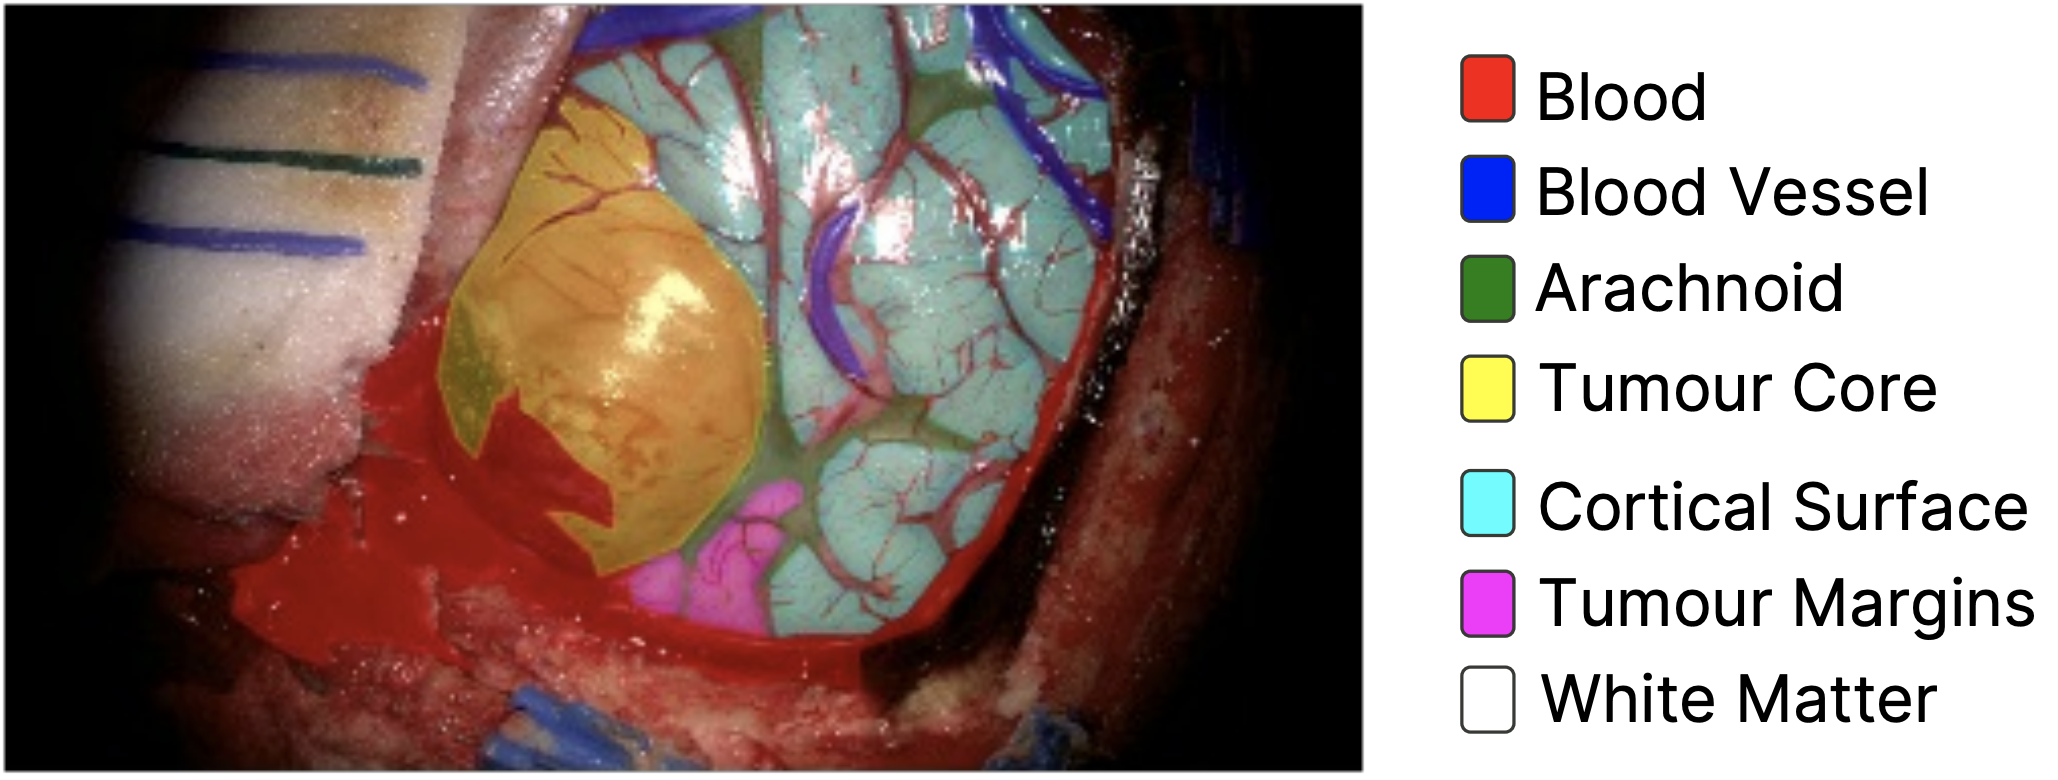
\includegraphics[width=\textwidth]{figures/label.png}
    \caption{A microscope image and its corresponding label.}
    \label{fig:label}
\end{minipage}
\end{figure}

\begin{figure}[h]
\centering
\begin{minipage}[h]{0.7\textwidth}
    \centering
    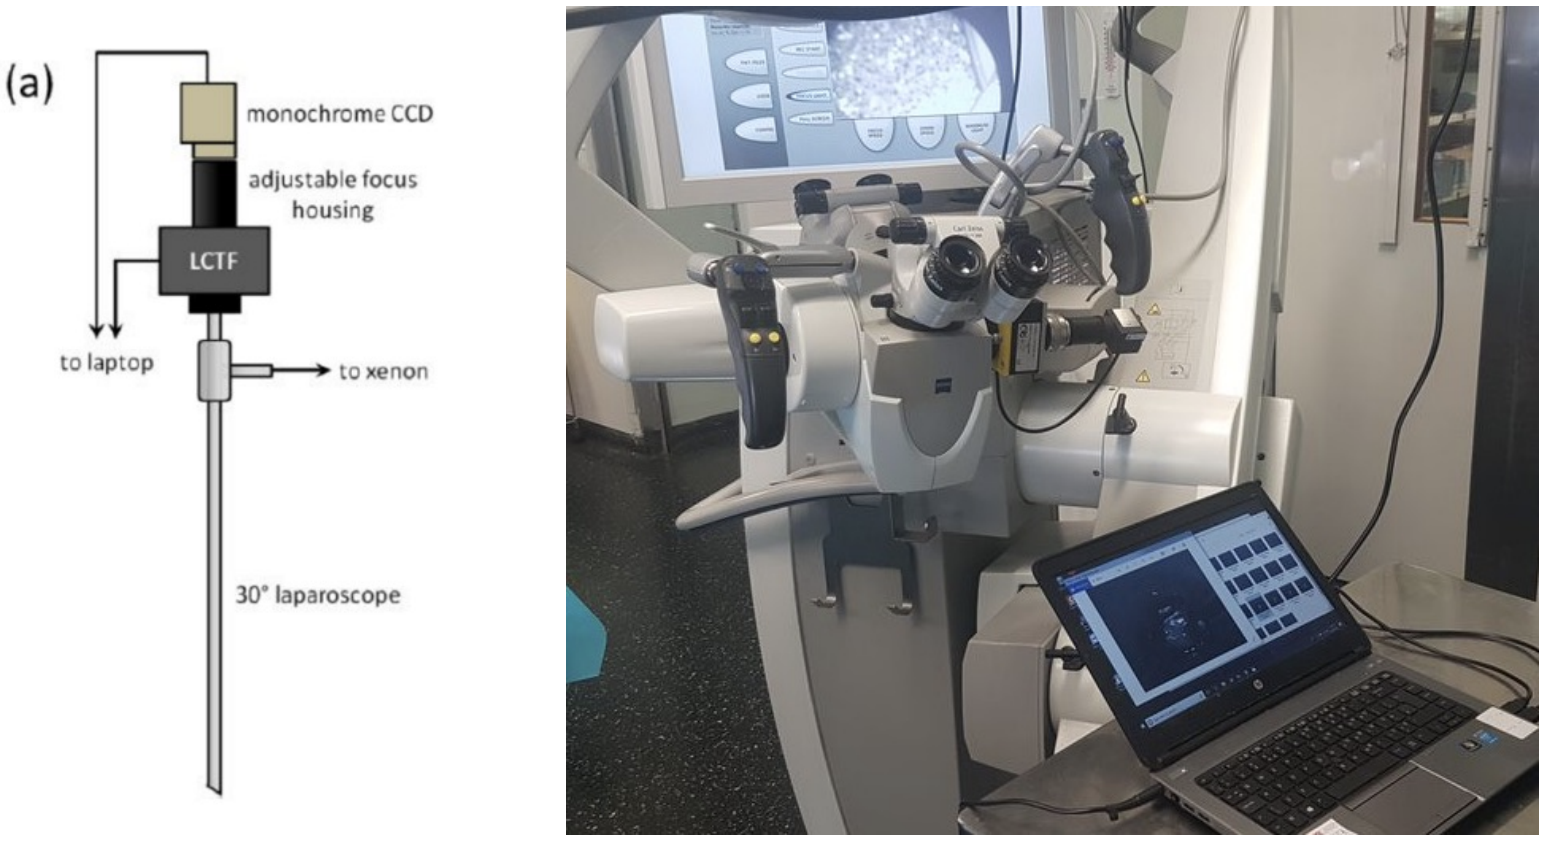
\includegraphics[width=\textwidth]{figures/camera-system.png}
    \caption{Image capture system diagram (left) and its photo in the operating room (right).}
    \label{fig:camera-system}
\end{minipage}
\end{figure}


\section{Aim}

\paragraph{}
In this project, we explored the use of multi-spectral imaging based on the dataset to analyse neurosurgical environments as a classification problem. While the dataset acquired is valuable, further work remains to be done as only the images from the microscope are labelled. Analysis of the spectral image stack would require applying the labels to them, which can be done by registering the microscope image to the spectral image stack. Therefore, the main question of this project is, \textit{"How can we prepare the raw image and label data into a usable format for further analysis?"}.


\section{Challenges}

\paragraph{}
\textbf{Displacement} --- During surgery, respiratory movement and haemodynamics cause the structure on the brain's surface to contract and dilate. Additionally, the spectral image of each wavelength is captured sequentially, with an acquisition time of either 50 or 200 ms. As a result, objects of interest, such as blood vessels or tissues captured in one spectral image, may appear further apart or closer together in other spectral images of the same stack. Ideally, we want these objects of interest to be at the same position regardless of which spectral image it is, as we only have a single label for the whole stack. A video that visualises displacement throughout the spectral image stack can be seen through the link in appendix \ref{appendix:tissue-disp}.


\paragraph{}
\textbf{Colour and Contrast} --- Another important problem is that the system used to acquire the microscope images and the spectral image stacks were inherently different. The system that acquires the microscope images produces a colour image with \acrshort{rgb} channels, whereas the spectral image system produces a monochromatic image based on the object's intensity at a given wavelength, as seen in figure \ref{fig:colour-spectral}. Moreover, while \acrshort{rgb} lies on the spectrum range of the spectral image, one single colour cannot be directly mapped into a single wavelength, for example, the colour green to 550 nm. Also, we expect the intensity distribution between each wavelength to differ as different objects emit or reflect different wavelengths with different values. An objective measurement using metrics to find the similarity of images, either between microscope to spectral stack or between images of the same stack, will not yield a perfect similarity.

\begin{figure}[h]
\centering
\begin{minipage}[h]{\textwidth}
    \centering
    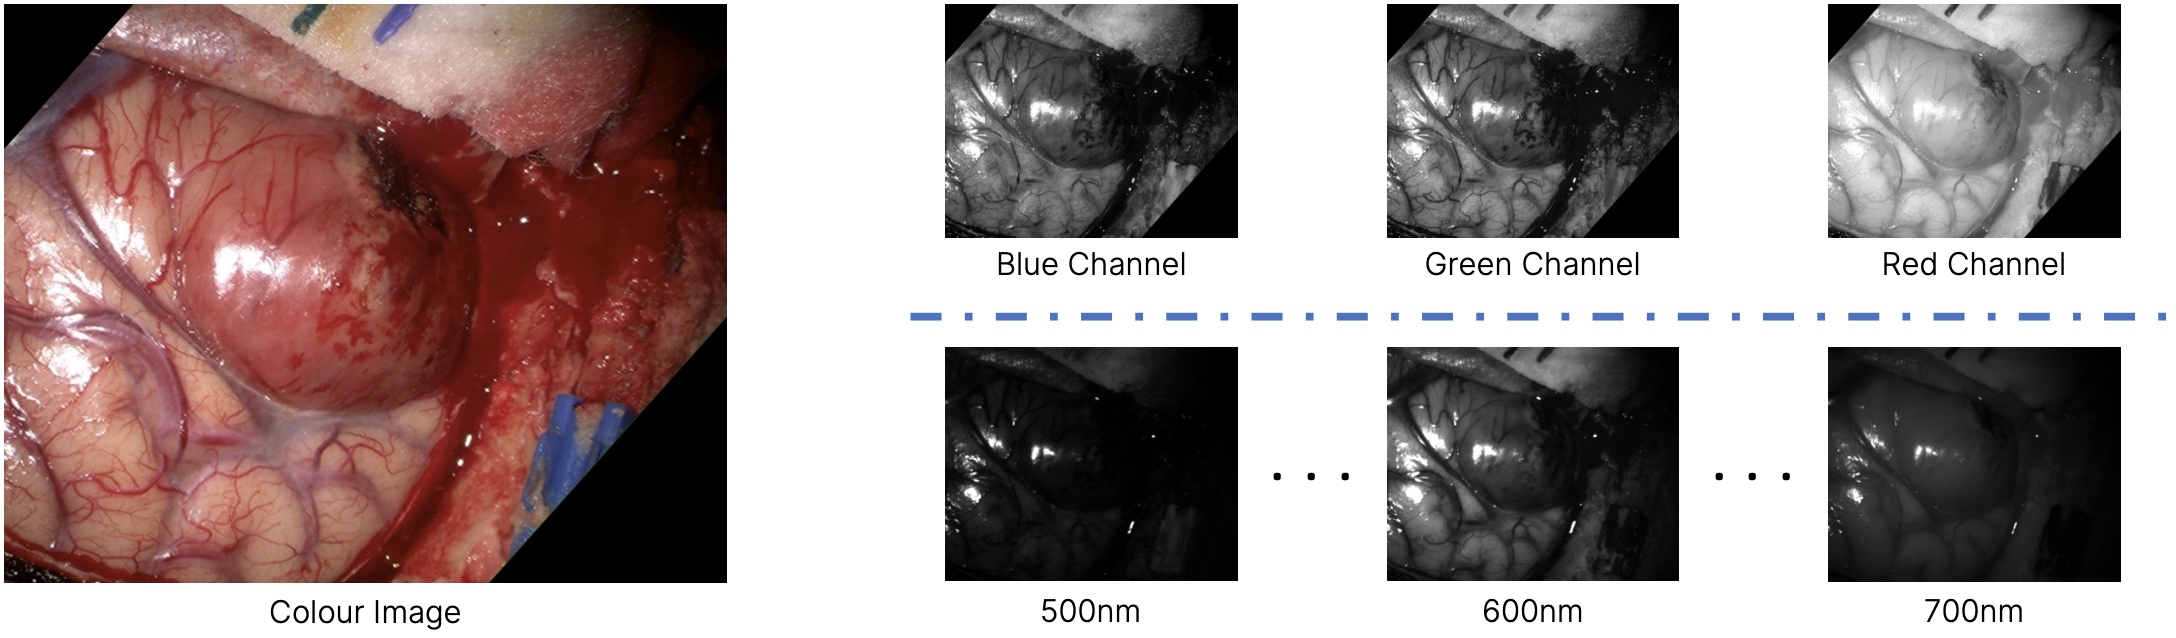
\includegraphics[width=0.8\textwidth]{figures/colour-spectral.png}
    \caption{Image of a scene with its microscope image (left), corresponding RGB channels (right, top row) and three spectral images (right, bottom row).}
    \label{fig:colour-spectral}
\end{minipage}
\end{figure}

\paragraph{}
\textbf{Perspective} --- A further issue in registering the microscope image to the spectral image stack is their perspective differences. While both camera systems may capture the scene simultaneously, they are positioned in different locations in the surgery room. Therefore, the image from one system may appear transformed and/or flipped compared to another, as shown in figure \ref{fig:plain-mic-spec}. In our case, we need images from both systems to be aligned, as the labels are associated with the microscope images but not the spectral image stacks.

\begin{figure}[H]
\centering
\begin{minipage}[h]{\textwidth}
    \centering
    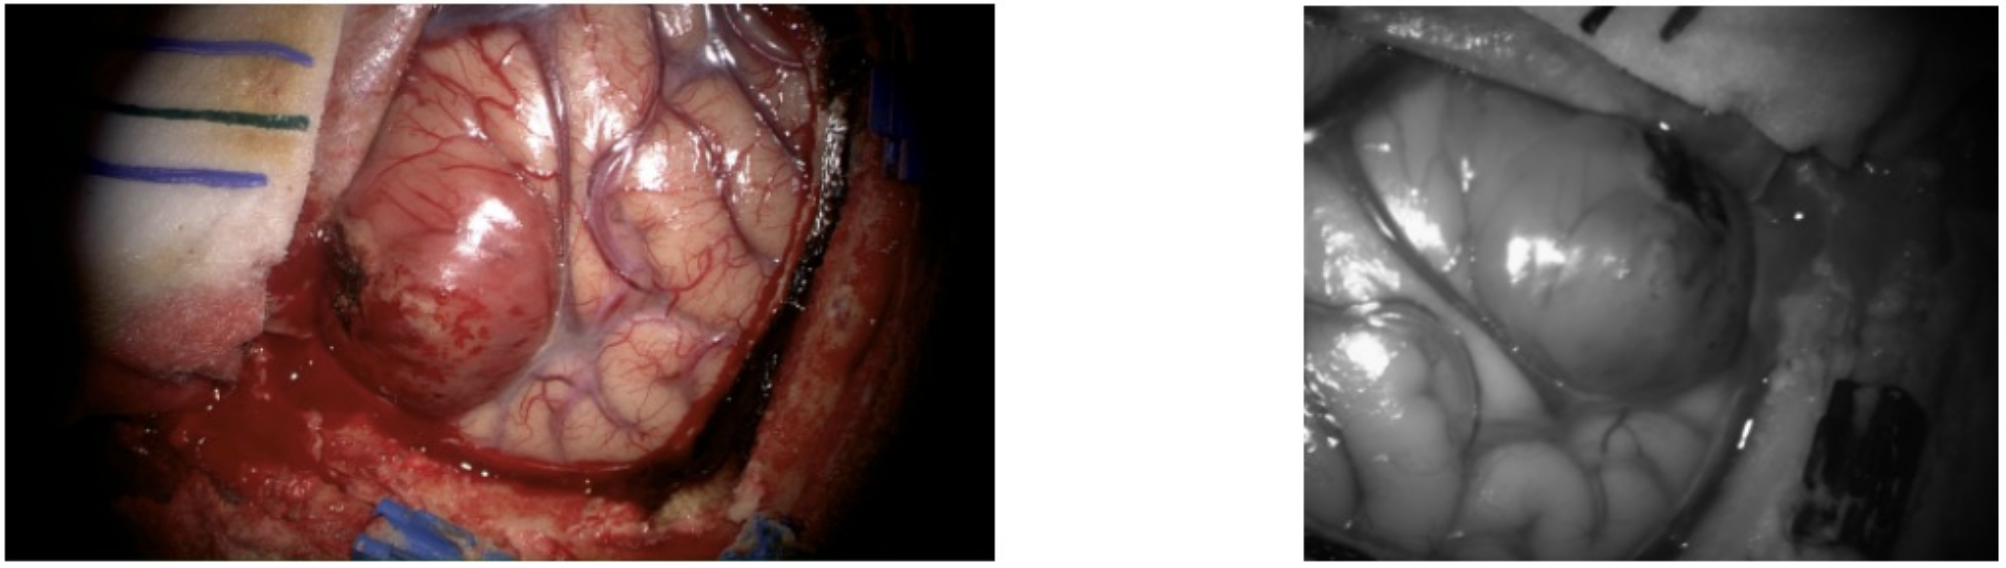
\includegraphics[width=0.6\textwidth]{figures/plain-mic-spec.png}
    \caption{A microscope image (left) and a spectral image(right) from the same scene.}
    \label{fig:plain-mic-spec}
\end{minipage}
\end{figure}

%%%%%%%%%%%%%%%%%%%%%%%%%%%%%%%%%%%%
\chapter{Literature Review}

\paragraph{}
The use of multi-spectral imaging relies on the idea that when radiated using a spectrum of electromagnetic waves, different materials will react differently \cite{wu_review_2022}. Based on these reactions, the detector can acquire distinct electromagnetic radiation values coming from each material through emission or reflection. A channel in a multi-spectral image can then be defined as the value reflected off the material given a single electromagnetic band. Spatial information is obtained by acquiring the reflection on a planar detector, creating a two-dimensional image. Then, spectral information is acquired by repeating the same process with different bands, essentially adding more channels to the image, resulting in a cube-like image structure where each pixel stores the information of multiple electromagnetic bands. 

\paragraph{}
Research on the use of multi-spectral images has been conducted across several domains. It has found its use in art science to identify paints used on a painting \cite{pelagotti_multispectral_2008} and enhance details of cave wall paintings \cite{legnaioli_recovery_2013}. Many multi-spectral imaging implementations have also been found in agriculture, ranging from terrain sensing \cite{berni_thermal_2009} to evaluating food safety and quality \cite{qin_hyperspectral_2013}.

\paragraph{}
Medical imaging also benefits from the use of multi-spectral imaging. The type of tissues and their content, such as blood, water, melanin, fat and yellow pigments, affect the optical coefficients when radiated by electromagnetic bands ranging from 400nm to 1300nm \cite{jacques_optical_2013}. Furthermore, several research based on the analysis of multi-spectral images has been conducted in the medical domain. Multi-spectral image analysis has been shown to identify residual tumours present after breast cancer resection \cite{panasyuk_medical_2007}, evaluate the development of bruises on the skin \cite{randeberg_hyperspectral_2006} and classify liver tissues \cite{hashimoto_tissue_2017}.

\section{MSI in Neurosurgery}
\paragraph{}
Neurosurgery is a branch of surgery that concerns the treatment of diseases affecting the nervous system, such as the brain and spinal cord. Medical staff that specialise in neurosurgery is called a neurosurgeon. Neurosurgeons handle many neurological diseases as a part of the hospital team; one of these cases is brain tumours. About 12,300 people are diagnosed yearly with benign or malignant brain tumours \cite{cruk_brain_2023}. Several strategies are used to treat brain tumours, including radiotherapy using high-energy X-rays and chemotherapy using anti-cancer drugs. However, surgery is the main treatment for most tumours \cite{cruk_brain_2023, bush_current_2017}, and the relevant information available is crucial in maximising surgical success.

\paragraph{}
Some imaging modalities, such as computed tomography (CT) and magnetic resonance imaging (MRI), have been commonly used to diagnose and treat brain tumours. Although information acquired by these imaging modalities is beneficial, most images are only used in decision-making before surgery as they have some disadvantages. One of the main drawbacks of CT and MRI is the need for a specialised room for their procedure due to the size of the machines. Health professionals must also wear heavy lead-grown to protect them from X-ray radiation throughout CT procedures. Furthermore, the use of strong magnets in MRI limits the use of equipment made out of metal as they can be attracted to the machine.

\paragraph{}
Other challenges may be faced when using pre-operative image data. One of the neurosurgeon’s tasks in a surgical procedure is to map the actual location of the tumour relative to the references based on its position in the image. However, while the information is enough for the surgeon to find the general region, the tumour's exact size and boundary might be difficult to locate as the patient’s body might move over the procedure known as brain shift \cite{gerard_brain_2017}. Multi-spectral imaging solves the problems mentioned, as it offers a non-invasive technique with a smaller machine that can acquire spatial and spectral information during surgery.

\paragraph{}
Several publications have discussed the analysis of multi-spectral images for neurosurgery, especially in the cerebral region. Overall, the analyses that have been done on multi-spectral images can be categorised into two main areas: brain tissue metabolic and haemodynamic and brain cancer diagnosis \cite{wu_review_2022}. Brain tissue metabolic and haemodynamic concerns chemical changes in the cerebral tissue, such as oxygenation. One study showed cerebral oxygenation and metabolism can be obtained from multi-spectral images based on near-infrared bands \cite{nguyen_hyperspectral_2019}. Most research focused on classifying tissue types for brain cancer diagnosis, ultimately identifying the cancerous area and its boundary. The use of visible and near-infrared bands is shown to be suitable for achieving segmentation \cite{fabelo_helicoid_2016}. 

\section{Medical Image Registration}
\paragraph{}
Image registration is a technique used to align two images. The main motivation for registration is to understand the context of photos that may not necessarily be the same but share some common information. In a review by Maintz and Viergever \cite{maintz_survey_1998}, the registration problem can be divided into several classifications. Some important criteria are the dimensionality of the data and whether we are working in 2D or 3D space. Another criterion is the nature of the transformation, such as rigid, affine or deformable. The modality of the data is also important, as registering images from different modalities would need a larger effort.

\paragraph{}
In medical settings, Oliveira and Tavares \cite{oliveira_medical_2014} concluded that feature-based registration can be generalised into several steps. In the first step, a pair of images is prepared either from itself or from a frame of a moving image. Afterwards, features are extracted from the images. Once extracted, the correspondences or pairs between features are determined as a cost function. Thus, finding the optimum transformation to register the image can be done by minimising the cost of correspondence.


%%%%%%%%%%%%%%%%%%%%%%%%%%%%%%%%%%%%
\chapter{Methodology}

\paragraph{}
The overall process is divided into two main stages. In the first stage, the raw data that has been acquired are put through a preprocessing pipeline that aligns spectral image stacks with the microscope images and, therefore, the labels. The second stage is to conduct an analysis of these images to prove the significance of having the labels registered with the spectral image stacks.

\section{Registration}
\paragraph{}
In this section, we will try to resolve the challenges of this project. The purpose of this section is to devise our registration process and discuss how each step of the process relates to the challenges. The output of this stage would be a registration pipeline that aligns the microscope images and the spectral image stack.

\subsection{Stack Registration}
\paragraph{}
Our first challenge that needs to be solved is the displacement of the brain surface on spectral images from the same stack. If we compare the images from one to another, the structures of images in the spectral image stack are all similar. A video going through all images from the stack can be seen via the link in appendix \ref{appendix:tissue-disp}. We can see from the video that the structure of the brain stays the same, but the regions move independently. The relation between the images hints that the type of transformation to register them is deformable.

\paragraph{}
Before we do the registration, we must select an image from the stack as our reference image that will act as the registration target for the rest of the stack. Ideally, the reference image would have the most notable structure than the rest of the stack to have the most amount of features. In our dataset, each spectral image stack has 29 channels. To select the reference image, we calculate the variance of each channel and then select the image with the highest variance. The idea is that an image with a high variance will have the most varying intensity. If we do this procedure for all runs in all patients, we can get the optimal channel for our reference image. In our case, the reference image is the 560 nm image.

\paragraph{}
The spectral image stack is then registered to the reference image using a hybrid non-rigid registration technique by Du \etal \cite{du_robust_2015} based on \acrfull{pfn} and \acrfull{dlk}, modified form of Lucas-Kanade's method \cite{lucas_iterative_1981}, by Zhu \etal \cite{zhu_fast_2009}. The technique was chosen as it has input and output types as our stack registration process. It also offers a graphical user interface application that is accessible to people with minimal programming knowledge.

\paragraph{}
The process starts with creating a 2D triangular geometric mesh model based on a method by Pilet \etal \cite{pilet_fast_2008}. For any point in the image, it can be defined as a barycentric coordinate $(b_i, b_j, b_k)$ from one triangle. Then, finding the transformation of the image can be done by observing the movement of feature points and estimating the transformation of the mesh' triangles based on the difference. In the figure \ref{fig:pfnlk-mesh}, you can see green meshes on top of the image to be registered.

\vspace{0.2cm}
\begin{figure}[h]
\centering
\begin{minipage}[h]{0.5\textwidth}
    \centering
    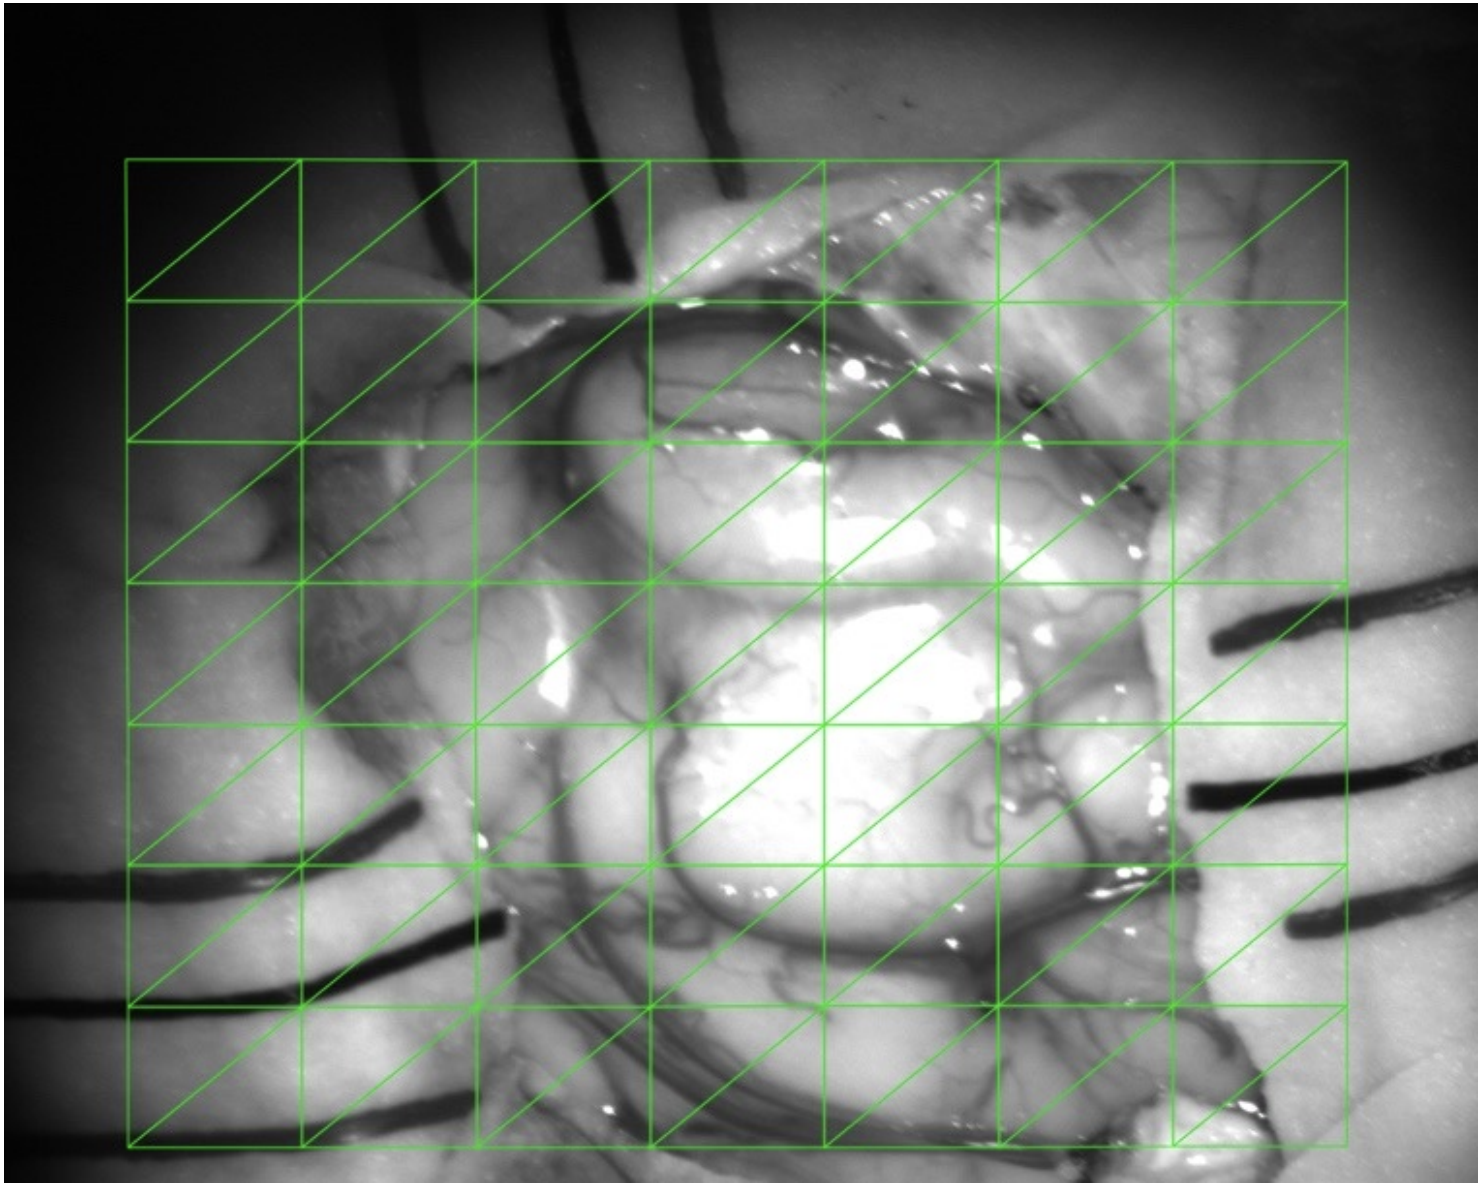
\includegraphics[width=\textwidth]{figures/pfnlk-mesh.png}
    \caption{Triangular mesh on top of a spectral image.}
    \label{fig:pfnlk-mesh}
\end{minipage}
\end{figure}

\paragraph{}
As mentioned earlier, we need feature points to estimate the transformation between two images. A feature point is a distinctive point or part of an image that can be easily identifiable and attributed to that specific image. If two images are similar, it is possible that they share some common feature points. While they can be chosen manually, feature points are often detected using a descriptor. Once the feature points are extracted from two images, we can determine the positional difference of a point by finding a pair of points in the source and target images that describe the same feature, also known as correspondence. It was mentioned in \cite{du_robust_2015} that the hybrid registration technique is agnostic on the type of feature extraction and correspondence that is used.

\paragraph{}
To register the geometric mesh once after computing the correspondences, \cite{du_robust_2015} discusses two methods, \acrshort{pfn} and \acrshort{dlk}. In \acrshort{pfn}, if $S$ is the state of the mesh in a vector form, the objective function $\varepsilon_F (S)$ that we are trying to minimise would be

\begin{equation}
    \varepsilon_F (S) = \lambda \varepsilon_R (S) + \varepsilon_C (S)
\end{equation}

where $\varepsilon_R (S)$ is a rotationally invariant deformation energy of the mesh with $\lambda$ as the the controlling constant and $\varepsilon_C (S)$ as the correspondence energy \cite{du_robust_2015, pilet_fast_2008}. Whereas in the modified \acrshort{dlk} \cite{zhu_fast_2009}, the objective function to be minimised is

\begin{equation}
    \varepsilon_F (S) = \lambda \varepsilon_R (S) + \varepsilon_{SCV} (S)
\end{equation}

where $\varepsilon_{SCV} (S)$ is the correspondence energy metric called the sum of conditional variance (SCV) \cite{pickering_new_2009}, a newer similarity metric. Notice that the correspondence energy differs from the proposed method by \cite{zhu_fast_2009}, where they use the sum of squared differences (SSD) instead of SCV. Results from \cite{du_robust_2015} show that combining both methods produced better registration outcomes than the methods alone. Thus, the hybrid method \acrshort{pfn} and \acrshort{dlk} or PFNLK is chosen as the method for stack registration.

\paragraph{}
In this step, most of the parameters are set to their default value. The highlight removal feature is not used, and we set the threshold value to 255. We use scale-invariant feature transform (SIFT) \cite{lowe_object_1999} to extract the features from the image pair. The features are then passed on to the hybrid PFNLK method. When finished, a new directory containing the registered spectral images will appear.


\subsection{Global Registration}

\subsubsection{Inferring RGB from MSI}
\paragraph{}
Colour and contrast are one of the main problems of registering the microscope image to the spectral image stack. As mentioned in one of the challenges, directly registering the images would not be ideal as they have different value distributions. One way to solve this problem is by inferring an \acrshort{rgb} image from the spectral image stack. This is possible as \acrshort{rgb} itself is a form of aggregation of several wavelengths in the visible light range. Hence, the registration process would be between images of the same channel, e.g., the microscope image's blue channel, to the inferred image's blue channel.

\paragraph{}
To infer an \acrshort{rgb}, we use an autoencoder neural network model comprised of an encoder and a decoder. An example of an autoencoder can be seen in figure \ref{fig:autoencoder}. In autoencoder, the goal is to encode the input into latent variables and then decode or recreate the input based on the latent variables. The encoder comprises four $3 \times 3$ convolution layers chain, resulting in 64 latent variables. The decoder also comprises a chain of four $3 \times 3$ convolution layers but transforms the latent variables into a monochromatic image.

\begin{figure}[h]
\centering
\begin{minipage}[h]{0.8\textwidth}
    \centering
    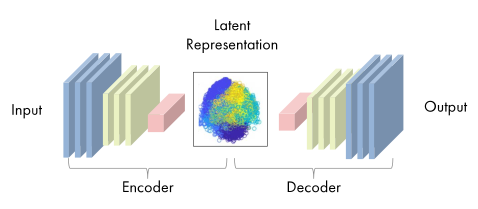
\includegraphics[width=\textwidth]{figures/autoencoder.png}
    \caption{An example of an autoencoder architecture \cite{mathworks_autoencoders_nodate}.}
    \label{fig:autoencoder}
\end{minipage}
\end{figure}

\paragraph{}
The model is trained by having spectral images as its inputs. When the model is fully trained, we expect the latent variables to represent the features of a spectral image. To infer a channel of \acrshort{rgb}, we can calculate the average values of the latent variable. For example, to infer a blue channel, we can get the latent variables of spectral images from 460 nm to 540 nm and then average the values. The result is a monochromatic image representing channels of \acrshort{rgb}, which can be seen in figure \ref{fig:inferred-rgb}.

\vspace{0.2cm}
\begin{figure}[h]
\centering
\begin{minipage}[h]{\textwidth}
    \centering
    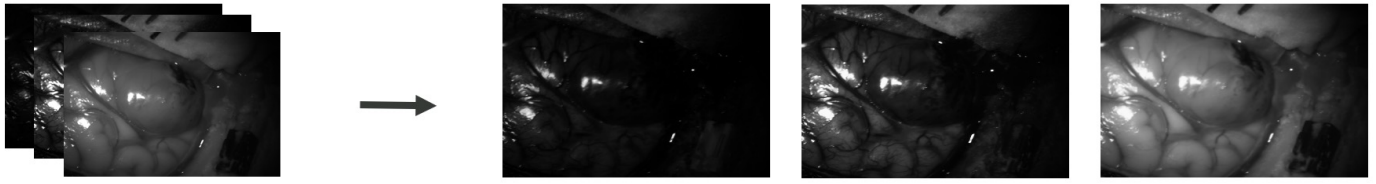
\includegraphics[width=\textwidth]{figures/inferred-rgb.png}
    \caption{Stack images (left) and inferred RGB images (right).}
    \label{fig:inferred-rgb}
\end{minipage}
\end{figure}

\subsubsection{Registering microscope image to spectral image}
\paragraph{}
The next step would be registering the microscope image to the inferred image. In this step, the microscope image is transformed to become as if it is taken from the same perspective as the spectral image stack. There are multiple ways to register the images. Compared to the stack registration, the transformation will have a larger rotation angle with some flips, as shown in figure \ref{fig:pers-corr}. The type of transformation indicates that a non-rigid technique would be suitable for this problem. This project evaluates two main registration methods: projective transformation by estimating the homography matrix and an affine transformation based on the least-squares solution of feature correspondences.

\begin{figure}[h]
\centering
\begin{minipage}[h]{0.9\textwidth}
    \centering
    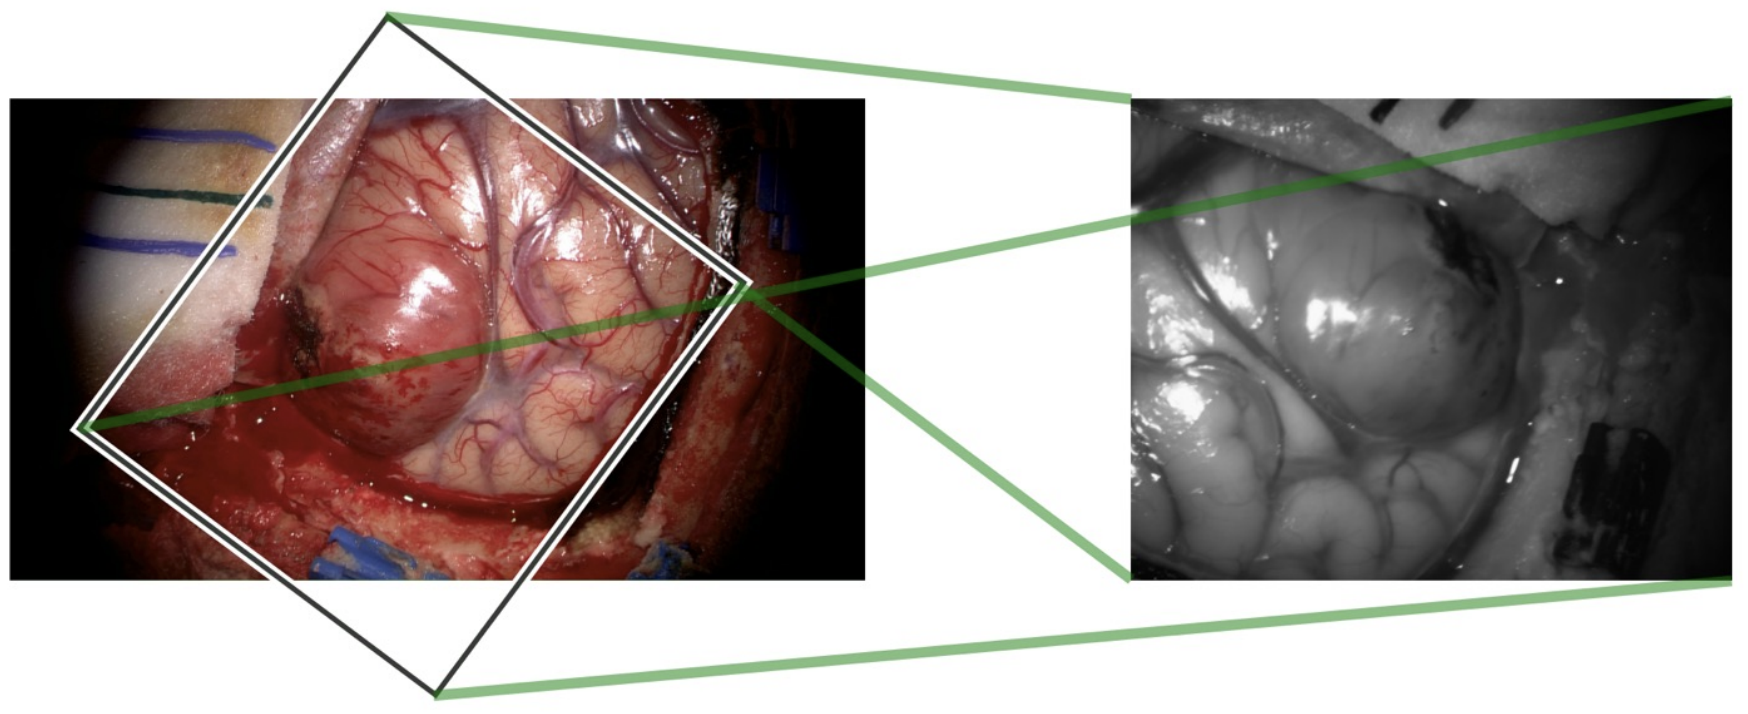
\includegraphics[width=\textwidth]{figures/pers-corr.png}
    \caption{Correspondences between a microscope and a spectral image from the same scene.}
    \label{fig:pers-corr}
\end{minipage}
\end{figure}

\paragraph{}
The homography matrix is a transformation matrix that maps a point projected on one plane to another plane. If $\textbf{H}$ is the homography matrix, then the relation between points would be

\begin{equation}
    s
    \begin{bmatrix}
    x'_i \\ y'_i
    \end{bmatrix}
    =
    \textbf{H}
    \begin{bmatrix}
    x_i \\ y_i
    \end{bmatrix}
\end{equation}

where $s$ is the scaling constant and $\textbf{H}$ is a $3 \times 3$ matrix. If

\begin{equation}
    \textbf{H}
    =
    \begin{bmatrix}
    h_{11} & h_{12} & h_{13} \\ h_{21} & h_{22} & h_{23} \\h_{31} & h_{32} & h_{33}
    \end{bmatrix}
\end{equation}

then estimating $\textbf{H}$ can done by minimising

\begin{equation}
    \sum_i
    {\biggl(x'_i - \frac{h_{11}x_i + h_{12}y_i + h_{13}}{h_{31}x_i + h_{32}y_i + h_{33}}\biggl)}^2
    +
    {\biggl(y'_i - \frac{h_{21}x_i + h_{22}y_i + h_{23}}{h_{31}x_i + h_{32}y_i + h_{33}}\biggl)}^2
\end{equation}


\paragraph{}
Affine transformation is a matrix comprising 4 basic transformations: rotation, scale, translation and shear. The relation between a point $x, y$ and the resulting transformation $x', y'$ with an affine transformation $\textbf{M}$ is

\begin{equation}
    \begin{bmatrix}
    x'_i \\ y'_i \\ 1
    \end{bmatrix}
    =
    \textbf{M}
    \begin{bmatrix}
    x_i \\ y_i \\ 1
    \end{bmatrix}
\end{equation}

where

\begin{equation}
    \textbf{M}
    =
    \begin{bmatrix}
    a_{11} & a_{12} & a_{13} \\ a_{21} & a_{22} & a_{23} \\ 0 & 0 & 1
    \end{bmatrix}
\end{equation}

To estimate the affine transformation matrix, we can use the least-squares solutions of

\begin{equation}
    \textbf{M}
    \begin{bmatrix}
    x_i \\ y_i \\ 1
    \end{bmatrix}
    =
    \begin{bmatrix}
    x'_i \\ y'_i \\ 1
    \end{bmatrix}
\end{equation}

by finding

\begin{equation}
    \textbf{M}^T
    \textbf{M}
    \begin{bmatrix}
    x_i \\ y_i \\ 1
    \end{bmatrix}
    =
    \textbf{M}^T
    \begin{bmatrix}
    x'_i \\ y'_i \\ 1
    \end{bmatrix}
\end{equation}

\paragraph{}
If we compare the methods that have been mentioned, we can see that they are quite similar, with both methods utilising a $3 \times 3$ transformation matrix. However, their difference lies in the third row of the transformation matrices. In the homography matrix, the third row affects the resulting transformation. Therefore, the affine transformation matrix retains line straightness and parallelism, whereas the homography matrix does not.


\subsection{Finer Registration}
\paragraph{}
At this point, the microscope image and the spectral image stack are roughly aligned. The structures of the microscope image should match the spectral image stack. However, if we compare the images closely in figure \ref{fig:fine-not-match}, some regions of the image might not align due to displacement of the surface tissue. The image is expected to not perfectly match as the microscope and spectral image stacks were taken at different times during the surgery.

\begin{figure}[h]
\centering
\begin{minipage}[h]{\textwidth}
    \centering
    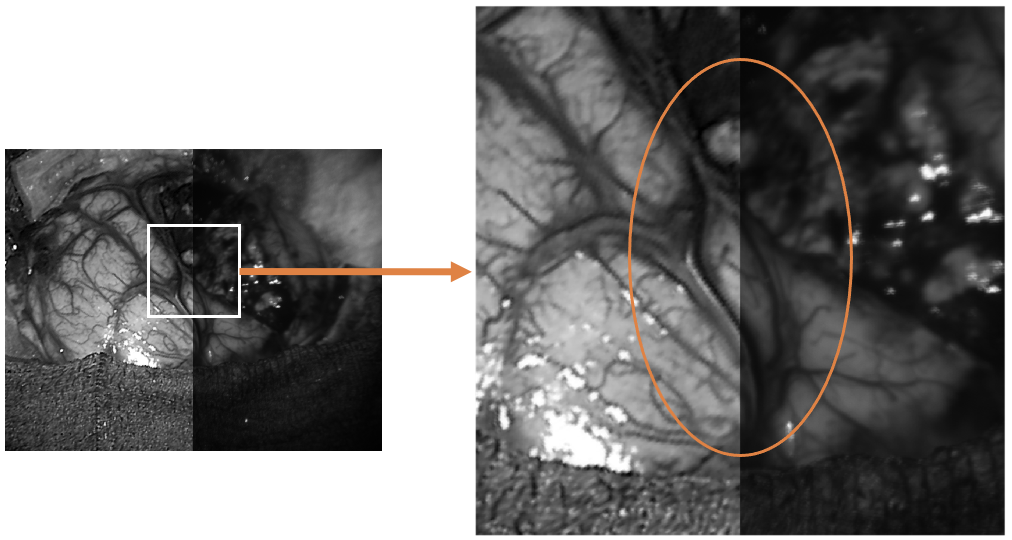
\includegraphics[width=0.8\textwidth]{figures/fine-not-match.png}
    \caption{A split image of microscope and spectral image (left) and a highlighted area with slight deformation (right).}
    \label{fig:fine-not-match}
\end{minipage}
\end{figure}

\paragraph{}
The type of transformation that is suitable for this task is a deformable registration method. While it is similar to stack registration, the main difference is that we only have to register the inferred \acrshort{rgb} image generated from the spectral image stack to the microscope image and then use the resulting registration deformation field for the rest of the image in the stack. The deformation field is a set of vectors defining a particular image's movement. Since we have to define the movement for all pixels, the deformation field would have the same dimension as the image it describes.

\paragraph{}
A deformable registration method called RANSAC-Flow by Shen \etal \cite{shen_ransac-flow_2020} is used for the last and finer registration. The method is a deep learning model split into two stages: coarse alignment by feature-based RANSAC \cite{fischler_random_1981} and fine alignment by local flow prediction. The course alignment process uses convolution-based feature extraction layers taken from ResNet architecture \cite{he_deep_2015} using pre-trained weights of ImageNet \cite{deng_imagenet_2009} and MoCo self-supervision \cite{he_momentum_2020}. Once the feature is extracted, a homography matrix is estimated using RANSAC. The model tries to minimise a loss function for the fine alignment between a pair of images $I_s$ and $I_t$. Given a reconstruction loss $\mathcal{L}_{\text{rec}}$, a matchability loss $\mathcal{L}_m$ and a cycle-consistency loss $\mathcal{L}_c$, the loss function is defined as

\begin{equation}
    \mathcal{L}(I_t, I_s) = 
    \mathcal{L}_{\text{rec}}(Is, It) +
    \lambda \mathcal{L}_m (Is, It) +
    \mu \mathcal{L}_c (Is, It)
\end{equation}

where $\lambda$ and $\mu$ as tunable hyperparameters \cite{shen_ransac-flow_2020}. The reconstruction loss uses structural index similarity measure (\acrshort{ssim}) \cite{wang_image_2004} to measure the similarity, while the cycle-consistency loss sets the cycle of layer inputs. The matchability loss then acts as weights to regulate the other two losses \cite{shen_ransac-flow_2020}.

\paragraph{}
Using the model, we can do the finer registration with the inferred \acrshort{rgb} as the source and microscope image as the target. The process results in a deformation field that can be used to register the spectral image stack. At the end of this stage, the microscope image should match the spectral image stack.


\subsection{Pipeline}
\paragraph{}
Initially, we have an \acrshort{rgb} microscope image and the spectral image stack of 29 wavelengths. To overcome the brain surface displacement, we do stack registration by estimating the deformable transformation using a hybrid method called PFNLK to align the stack across all wavelengths. Before registering the microscope image to the spectral image stack of the same scene, we infer an \acrshort{rgb} representation of the spectral image stack so that the registration will be between the same type of images. After the microscope image is aligned, a finer registration process is done to align minor image regions. As the labels correspond to the microscope image, we would only need to apply the same transformation as the microscope image to register the label. Combining all the techniques mentioned, the resulting pipeline can be seen in figure \ref{fig:pipeline}.

\vspace{0.2cm}
\begin{figure}[h]
\centering
\begin{minipage}[h]{\textwidth}
    \centering
    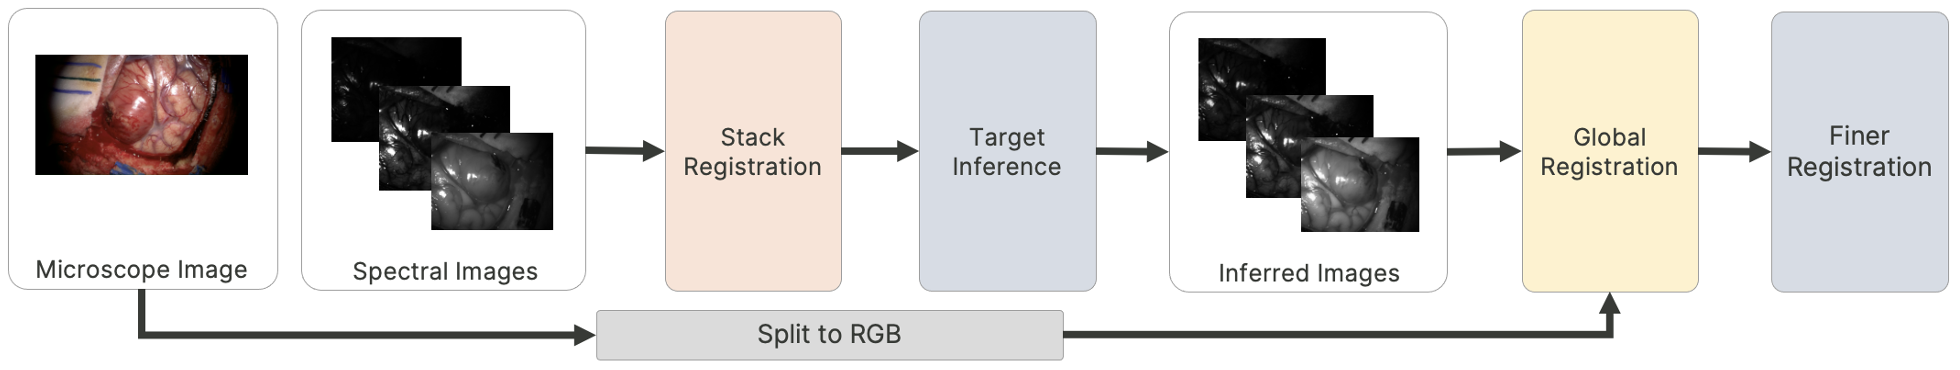
\includegraphics[width=\textwidth]{figures/pipeline.png}
    \caption{The overall registration pipeline.}
    \label{fig:pipeline}
\end{minipage}
\end{figure}


\section{Image Analysis}
\paragraph{}
After aligning the spectral image stack with labels, we can analyse objects based on their spectral values according to their types. In our dataset, nine objects are identified by the labels. The objects are blood, blood vessels, arachnoid, tumour core, cortical surface, tumour margins, white matter, dura and bone. There might be some regions of the image that are not labelled. In this case, we assign them as unlabelled.

\paragraph{}
From 49 patients with 5-16 scenes each, we took 20 scenes for analysis. The criteria of the scenes that we took are the spectral image taken with 50 ms exposure time. We also took scenes where the tumour core was not resected yet. Lastly, we only took one scene from each patient, so the microscope images and spectral image stacks were unique. Once selected, the scenes were randomly divided into training and testing data with a 70-30 split. This gives us 14 training scenes and 6 testing scenes.

\paragraph{}
The common way to do classification or image segmentation is to train a learning model. Based on the model's architecture, it can be divided into two categories. The first one is the classical machine learning (\acrshort{ml}) model. In classical ML, the goal is to tune the parameters of a or some mathematical function. The simplest classical ML model is the linear regression, where we fit the data to find the line gradient and a bias. Another model, such as naive Bayes, uses the probability and independence of the features derived from a Bayesian network to determine the model's output. The second category of learning models is models based on interconnected neural network layers (\acrshort{nn}). Instead of a mathematical function, it takes the inputs, multiplies them by tunable weights and then adds the bias. The resulting values are then passed through an activation layer and transformed into the desired domain. In this project, we experimented with learning models from both categories. For classical \acrshort{ml}, we fit the data using XGBoost \cite{chen_xgboost_2016} and for \acrshort{nn}, we use U-Net \cite{ronneberger_u-net_2015} architecture.

\subsection{XGBoost}
\paragraph{}
XGBoost is a gradient-boosting library that offers high-level API for model training \cite{chen_xgboost_2016}. The most basic component of XGBoost is the decision tree model. A decision tree comprises two types of nodes: the decision node and the end node. The decision node forks a path into two child nodes based on certain criteria, while the end node gives us the decision tree result. For an input, the path starts at the first decision node, also called the root node. Based on the criteria, the path will then lead to one of the child nodes, which can be both decision and end nodes. If the next node is a decision node, the path will continue, but if it is the end node, it will return the prediction based on the value of the end node it gets to.

\paragraph{}
While a decision tree model can be used independently, many models utilise a collection of decision trees. Random forest (RF) \cite{breiman_random_2001} is an example of a model that uses multiple decision trees to establish a voting system, where the majority prediction of the trees is used as the prediction result of the model. However, XGBoost differs from RF as it uses a concept called boosting. Instead of using a proper decision tree, it uses a weak tree with a default maximum depth of six, which means a path will only go through a maximum of five decision nodes \cite{chen_xgboost_2016}.

\paragraph{}
The objective function for boosting is as follows

\begin{equation}
    \text{obj} =
    \sum_{i=1}^n l(y_i, \hat{y_i}^{(t)}) +
    \sum_{i=1}^t \omega (f_i)
\end{equation}

where $l(y_i, \hat{y_i}^{(t)})$ is a loss function and $\omega (f_i)$ is a regularisation term. Next, we define the prediction at $\hat{y_i}$ at step $t$ as

\begin{equation}
    \hat{y_i}^{(t)} =
    \sum_{i=1}^t f_k (x_i) =
    \hat{y_i}^{(t-1)} + f_t (x_i)
\end{equation}

so the objective function at step $t$ becomes

\begin{equation}
    \text{obj}^{(t)} =
    \sum_{i=1}^n l(y_i, \hat{y_i}^{(t-1)} + f_t (x_i)) +
    \omega (f_t) + \text{constant}
\end{equation}

Since we are using logistic loss, when substituted, the resulting objective function is

\begin{equation}
    \text{obj}^{(t)} =
    \sum_{i=1}^n 
    \biggl[
        g_i f_t (x_i) +
        \frac{1}{2} h_i f_t^2 (x_i)
    \biggr] +
    \omega (f_t)
\end{equation}

where

\begin{equation}
    g_i =
    \partial_{\hat{y_i}^{(t-1)}}
    l(y_i, \hat{y_i}^{(t-1)})
\end{equation}

\begin{equation}
    h_i =
    \partial_{\hat{y_i}^{(t-1)}}^2
    l(y_i, \hat{y_i}^{(t-1)})
\end{equation}

\paragraph{}
We used the method \textit{XGBClassifier} from the XGBoost library \cite{chen_xgboost_2016} with additional parameters for this project. The learning rate is set to the default value of $0.03$. The learning task of the model is set to logistic regression as a binary classification. The area under the curve is selected as the evaluation metric, and we set an early stopping round limit of 10, so the training will stop if the loss does not get lower after the $n$ number of iterations.

\paragraph{}
We must first reformat the data before fitting it into the gradient-boosting model. Initially, our spectral image stack is in the form $[ N, H, W, C]$ where $N$ is the number of scenes, $H, W$ is the height and width of the image, respectively, and $C$ is the number of channels in the image, which is 29. Moreover, the label image is in the form $[N, H, W, 1]$ where the number of channels is one. To make prediction easier, non-tumour labels are set to $0$, while tumour labels are set to $1$. Afterwards, we \textit{unsqueeze} the data so that the shape becomes $[N \times H \times W, C]$ for the spectral image stack and $[N \times H \times W, 1]$ for the label image.

\subsection{U-Net}
\paragraph{}
U-Net is a deep-learning architecture that was created to solve biomedical image segmentation. At the time, there were many approaches to solving image segmentation problems using convolutional neural networks (\acrshort{cnn}). However, Ronneberger \etal \cite{ronneberger_u-net_2015} argued that the available CNN models might not be suitable for biomedical image segmentation tasks, as they were trained using a large dataset, while the datasets for biomedical images were far smaller. Furthermore, the paper \cite{ronneberger_u-net_2015} also mentioned remarks made by \cite{dosovitskiy_discriminative_2015} that highlight the importance of data augmentation for biomedical images to simulate variance and extend the image collection size.

\paragraph{}
The U-Net model introduces a U-shaped architecture where images from earlier stages of the process are copied and cropped to be used in the latter stages. The input image can be a three-dimensional array of any size where the first and second indices are the image size, and the third axis corresponds to the number of channels. The model's output is an image with the same height and width, but the number of channels or the third dimension will be the same as the number of labels predicted.

\paragraph{}
Five main operations make up the U-Net architecture. The first is a $3 \times 3$ convolutional layer with a rectified linear unit (ReLU) activation function. This layer expands the number of channels from the input. The next operation is a copy and crop intermediary where the image is taken to a later stage. The third operation is a max-pool layer that downsamples the image into smaller heights and widths. The fourth operation is an upsampling layer that expands the size of the image. At the very end, a convolutional layer is used to determine the predicted output. Figure \ref{fig:unet} shows the whole process based on these operations.

\begin{figure}[h]
\centering
\begin{minipage}[h]{0.9\textwidth}
    \centering
    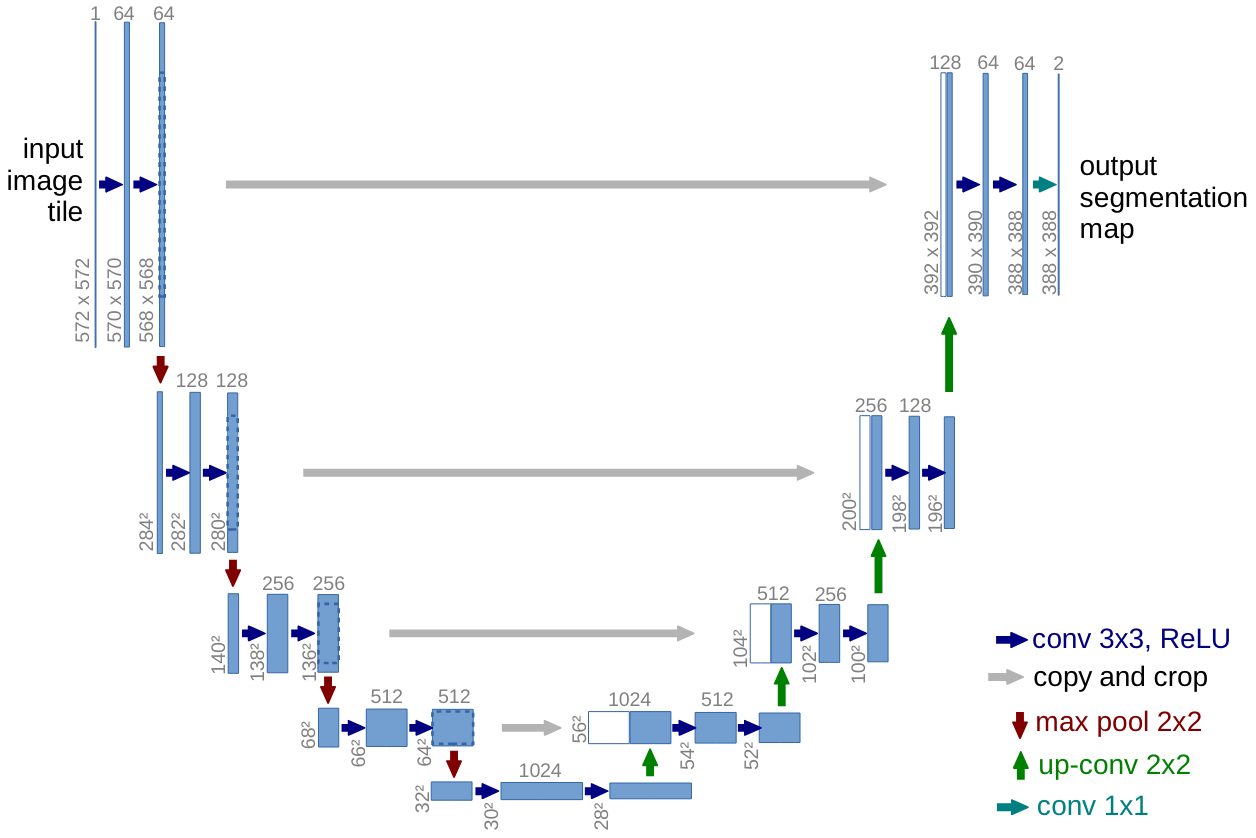
\includegraphics[width=\textwidth]{figures/unet.png}
    \caption{The U-Net architecture proposed by Ronneberger \etal \cite{ronneberger_u-net_2015}.}
    \label{fig:unet}
\end{minipage}
\end{figure}

\paragraph{}
For our project, the U-Net model was set up as following some parameters used in \cite{seidlitz_robust_2022}. We used the Adam \cite{kingma_adam_2017} optimisation algorithm to optimise the model. A loss function based on the Dice coefficient \cite{dice_measures_1945} was used to evaluate the model during training. Instead of using efficientnet-b5 encoder \cite{tan_efficientnet_2020} as used in \cite{seidlitz_robust_2022}, we found that ResNet101 \cite{he_deep_2015} performed better for our task, but we kept the source of pre-trained weights the same, which is the ImageNet \cite{deng_imagenet_2009}.

\paragraph{}
Before training the model, some changes need to be made to the dataset, conforming to the format of the model. At first, our format for the label images is $[N, H, W, 1]$, where we define the labels as integers on the last dimension. Unlabelled parts of the image were assigned zero as their value, and each label was assigned a non-zero number from one to nine. Based on the values assigned to the labels, we split the last dimension into three channels, each representing a particular category. The first channel has true values for unlabelled parts of the image or a value of zero. The second channel has true values for non-tumour labels or values of one to nine, except for four and six. The last channel has true values for tumour tissue and margins with values of four and six.

\paragraph{}
The training is set to 50 iterations or epochs. After each iteration, the model's intersection-over-union (IoU) score is calculated and used as the base for performance comparison. When the IoU score for an iteration is higher than the current highest score, it becomes the highest score and the model state is saved as into a \textit{.pth} file. In the first iteration, the learning rate was set to $1 \times 10^{-4}$. To make sure that the model fits into the extrema, the learning rate was then lowered two times at the 25\textsuperscript{th} and 40\textsuperscript{th} iteration to $5 \times 10^{-5}$ and $1 \times 10^{-5}$ respectively.


%%%%%%%%%%%%%%%%%%%%%%%%%%%%%%%%%%%%
\chapter{Results and Discussion}
\paragraph{}
In this chapter, we will discuss some results based on the registration process and analysis done on the acquired dataset. For each section, there will be two main types of evaluation. The first type is based on objective similarity metrics based on the kind of images evaluated, while the second is a visual assessment of the resulting process. The review by Oliveira \cite{oliveira_medical_2014} classified similarity metrics into two categories. The first is intensity-based similarity metrics, where the score is assessed based on the difference in pixel value or a function of localised pixels in an area between two images. The second is feature-based similarity measures, which are calculated based on the positional similarity of two corresponding features. In our project, we will focus on using intensity-based similarity metrics, as all registration techniques in the pipeline minimise a kind of feature-based similarity metric for their process. However, using intensity-based similarity metrics to compare multi-modal images by themselves is insufficient. Since they only offer similarity scores, they are useful when we are comparing two alignment techniques, but they cannot give us the score that we should aim for an ideal alignment. Therefore, we use visual assessment as a part of the evaluation.

\section{Registration}

\paragraph{}
As mentioned, the evaluation will be done by similarity metrics and visual assessment. Three similarity metrics were used to evaluate the registration techniques. As we were comparing the similarity between two different modalities or intensity distributions, the similarity metrics used should emphasise structural similarity. Therefore, we chose three similarity metrics: gradient magnitude similarity deviation (\acrshort{gmsd}) \cite{xue_gradient_2014}, \acrshort{ssim} and peak signal-to-noise ratio (\acrshort{psnr}).

\paragraph{}
The \acrshort{gmsd} is a full reference image quality assessment model based on gradient magnitude \cite{xue_gradient_2014}. The model utilises two techniques to make its assessment. Suppose that we have two images to compare, a reference image \boldit{r} and a deformed image \boldit{d}. The first step is calculating the images' gradient magnitude similarity (\acrshort{gms}). Using the Prewitt operator for each axis

\begin{equation}
    \textbf{h}_x = 
    \begin{bmatrix}
        \frac{1}{3} & 0 & -\frac{1}{3} \\
        \frac{1}{3} & 0 & -\frac{1}{3} \\
        \frac{1}{3} & 0 & -\frac{1}{3}
    \end{bmatrix}, \:
    \textbf{h}_y = 
    \begin{bmatrix}
        \frac{1}{3} & \frac{1}{3} & \frac{1}{3} \\
        0 & 0 & 0 \\
        -\frac{1}{3} & -\frac{1}{3} & -\frac{1}{3}
    \end{bmatrix}
\end{equation}

the magnitude of image \boldit{r} and \boldit{d} on location \textit{i} are defined as

\begin{equation}
    \textbf{m}_{r}(i) = 
    \sqrt{
        {(\textbf{r} \otimes \textbf{h}_x)}^2 (i)
        +
        {(\textbf{r} \otimes \textbf{h}_y)}^2 (i)
    }
\end{equation}

\begin{equation}
    \textbf{m}_{d}(i) = 
    \sqrt{
        {(\textbf{d} \otimes \textbf{h}_x)}^2 (i)
        +
        {(\textbf{d} \otimes \textbf{h}_y)}^2 (i)
    }
\end{equation}

which are then used to calculate the \acrshort{gms} as such

\begin{equation}
    \textit{\acrshort{gms}}(\textit{i}) =
    \frac
    {
        2 \textbf{m}_r(i) \textbf{m}_d(i) + c
    }
    {
        \textbf{m}_r^2 (i) + \textbf{m}_d^2 (i) + c
    }
\end{equation}

where $c = 0.0026$. The constant $c$ was selected based on the selected value in the paper \cite{xue_gradient_2014} that is used to regulate the denominator in case $\textbf{m}_r^2 (i) + \textbf{m}_d^2 (i) = 0$. Then, the gradient magnitude similarity mean (\acrshort{gmsm}) can be calculated as

\begin{equation}
    \textit{GMSM} =
    \frac{1}{N} \sum_{i=1}^N \textit{\acrshort{gms}}(\textit{i})
\end{equation}

the \acrshort{gmsd} is then defined as a function of \acrshort{gms} and \acrshort{gmsm}, where

\begin{equation}
    \textit{\acrshort{gmsd}} =
    \sqrt{
        \frac{1}{N} \sum_{i=1}^N
        {(\textit{GMS}(\textit{i}) - \textit{GMSM})}^2
    }
\end{equation}

\paragraph{}
The \acrshort{ssim} is an image quality assessment model based on the structural information between two images \cite{wang_image_2004}. The model measures the similarity of images using a combination of three comparisons: luminance, contrast and structure. First, we define the mean intensity of an image $\textbf{x}$ as

\begin{equation}
    \mu_x = \frac{1}{N} \sum_{i=1}^N x_i
\end{equation}

while the contrast is described as the standard deviation of the image, such that

\begin{equation}
    \sigma_x =
    {\Biggl(
        \frac{1}{N-1} \sum_{i=1}^N {(x_i - \mu_x)}^2
    \Biggl)}^{\frac{1}{2}}
\end{equation}

Then, the luminance measure is defined as

\begin{equation}
    l(\textbf{x},\textbf{y}) =
    \frac
        {2 \mu_x \mu_y + C_1}
        {\mu_x^2 + \mu_y^2 + C_1}
\end{equation}

in which $C_i = {(K_i L)}^2$, where $K_i \ll 1$ and $L$ is the dynamic range of pixel values \cite{wang_image_2004}. The contrast is compared by the function

\begin{equation}
    c(\textbf{x},\textbf{y}) =
    \frac
        {2 \sigma_x \sigma_y + C_2}
        {\sigma_x^2 + \sigma_y^2 + C_2}
\end{equation}

The structure comparison is then calculated as

\begin{equation}
    s(\textbf{x},\textbf{y}) =
    \frac
        {\sigma_{xy} + C_3}
        {\sigma_x \sigma_y + C_3}
\end{equation}

where the value of $\sigma_x \sigma_y$ is estimated through the equation

\begin{equation}
    \sigma_{xy} =
    \frac{1}{N-1} \sum_{i=1}^N
        (x_i - \mu_x)
        (y_i - \mu_y)
\end{equation}

By combining all three comparisons, the SSIM index is defined as

\begin{equation}
    \text{SSIM}(\textbf{x},\textbf{y}) =
        {[l(\textbf{x},\textbf{y})]}^\alpha \cdot
        {[c(\textbf{x},\textbf{y})]}^\beta \cdot
        {[s(\textbf{x},\textbf{y})]}^\gamma
\end{equation}

where $\alpha$, $\beta$ and $\gamma$ are set to a non-zero positive value to denote the significance of each comparison.

\paragraph{}
The \acrshort{psnr} is a ratio based on the logarithmic measure of the mean-square error (\acrshort{mse}) and maximum value between two images. Given a reference image $I_1$ and a second image $I_2$, both with dimension of $M \times N$, the \acrshort{mse} is defined as

\begin{equation}
    \text{\acrshort{mse}}(I_1, I_2) =
    \frac{1}{M \times N}
    \sum_{M,N} {[I_1(m,n) - I_2(m,n)]}^2
\end{equation}

Then, the \acrshort{psnr} is computed as

\begin{equation}
    \text{\acrshort{psnr}}(I_1, I_2) =
    10 \cdot \log_{10}
    \biggl( \frac{R^2}{\text{\acrshort{mse}}(I_1, I_2)} \biggl)
\end{equation}

where $R$ is the maximum value of the image range.

\paragraph{}
One thing to note is that different similarity metrics output different ranges of values. In \acrshort{gmsd}, a more similar image will result in a lower \acrshort{gmsd} value, while in \acrshort{mse} and \acrshort{psnr} case, the value will be higher.

\subsection{Stack Registration}
\paragraph{}
We devised a method to evaluate the stack registration process by comparing the similarity between each image of the spectral image stack before and after the registration process. The idea is that after the stack registration process, the similarity value between spectral stack images will be better compared to without the registration. Below are the results of the stack registration.

\begin{figure}
\centering
\begin{minipage}[h]{0.8\textwidth}
    \centering
    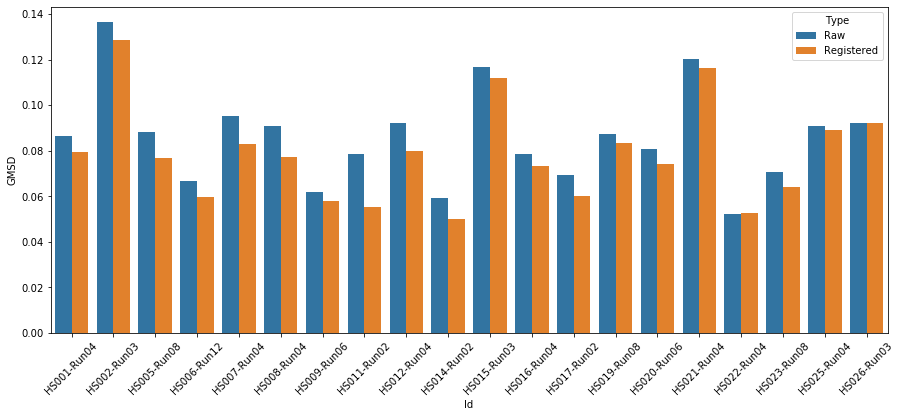
\includegraphics[width=\textwidth]{figures/stack-gmsd.png}
    \caption{Average \acrshort{gmsd} value of each stack before and after stack registration.}
    \label{fig:stack-gmsd}

    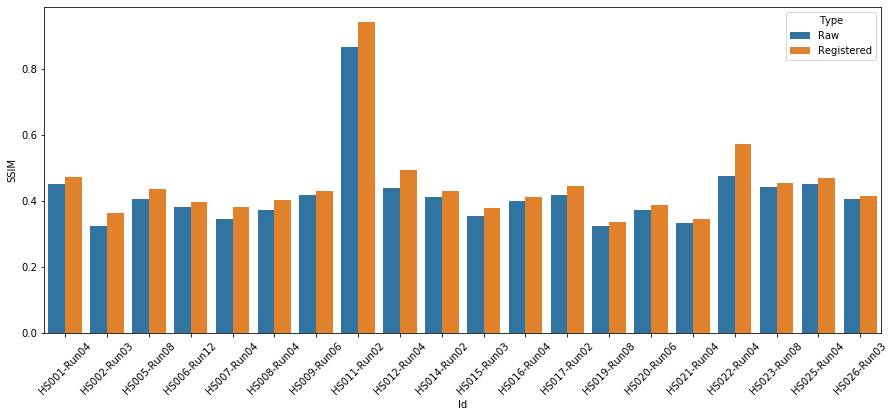
\includegraphics[width=\textwidth]{figures/stack-ssim.png}
    \caption{Average \acrshort{ssim} value of each stack before and after stack registration.}
    \label{fig:stack-ssim}

    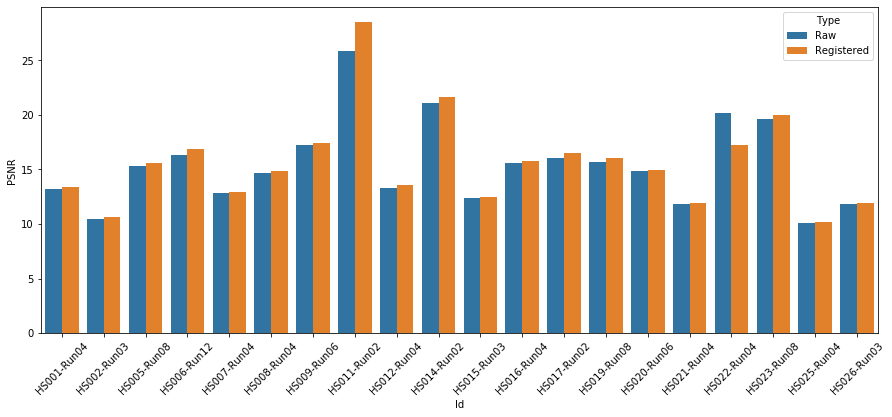
\includegraphics[width=\textwidth]{figures/stack-psnr.png}
    \caption{Average \acrshort{psnr} value of each stack before and after stack registration.}
    \label{fig:stack-psnr}
\end{minipage}
\end{figure}

\paragraph{}
The bar plots in figure \ref{fig:stack-gmsd}, \ref{fig:stack-psnr} and \ref{fig:stack-psnr} visualise the average difference in metrics value between unregistered and registered spectral image stacks. The x-axis denotes the scene's sample and run ID, and the y-axis denotes the average metrics value of the stack $\mu_{\text{stack}}$. To calculate the average metric value, each image in the spectral image stack was compared to other spectral images in the stack. For a spectral image stack $S$, an image of the stack $S_i$ and similarity metric $M$, the sum of the values was then averaged as follows

\begin{equation}
    \mu_{\text{stack}} =
    \frac
    {\sum\limits_{i=0}^n\sum\limits_{j=0}^n M(S_i, S_j)}
    {n^2}
\end{equation}

If a similarity metric is better when the value is higher, the metric value after the registration should also be higher and vice versa.

\paragraph{}
In figure \ref{fig:stack-gmsd}, we can see that for \acrshort{gmsd}, the $\mu_{\text{stack}}$ after registration are mostly lower except for HS026--Run03 where the average before and after registration did not vary by much. Since \acrshort{gmsd} value is lower when better, the figure shows that the stack was more similar after the registration. In figure \ref{fig:stack-ssim}, the $\mu_{\text{stack}}$ are higher for all scenes, which indicates the registration made the stack more structurally similar. In figure \ref{fig:stack-psnr}, the $\mu_{\text{stack}}$ are only marginally higher in most of the scenes. The exception in this figure can be seen at scene HS011--Run02, where the $\mu_{\text{stack}}$ is higher and at scene HS022--Run04, where the $\mu_{\text{stack}}$ is considerably lower after the registration.

\paragraph{}
The result of the stack registration can be seen through a video linked in appendix \ref{appendix:stack-reg-res}. The video shows an iteration through a spectral image stack before the stack registration on the left and the same stack after registration on the right. Multiple positional changes exist in the video where the stack is not registered. First, the whole scene moves perpendicular to the camera's line of sight. Second, it also shows that some regions, such as the tumour core at the centre-right of the scene, move independently compared to other regions. After the stack registration process, shown on the right side of the video, we can see that the positional changes mentioned are minimised.

\subsection{Global Registration}
\paragraph{}
For evaluating the global registration methods, we compared each channel of the microscope image with the inferred \acrshort{rgb} images using the same similarity metrics mentioned earlier. We then compared the results between the two registration methods, estimated homography matrix and estimated affine transformation matrix. The results of global registration are as follows

\begin{center}
\begin{table}[h]
\centering
\begin{tabular}{ c c c c c c c } 
 & \multicolumn{2}{c}{GMSD\^{}} & \multicolumn{2}{c}{SSIM*} & \multicolumn{2}{c}{PSNR*} \\
\hline
Channel & Proj & Affine & Proj & Affine & Proj & Affine \\
\hline
Red              & .102 & \textbf{.096} & .445 & \textbf{.475} & 13.828          & \textbf{14.53} \\
Green            & .126 & \textbf{.124} & .358 & \textbf{.359} & \textbf{12.846} & 12.750 \\
Blue             & .132 & \textbf{.131} & .233 & \textbf{.248} & 12.063          & \textbf{13.080} \\
\textbf{Average} & .120 & \textbf{.117} & .345 & \textbf{.360} & 12.912          & \textbf{13.455} \\
\hline
\end{tabular}

\vspace{0.2cm}
\^{} lower is better --- * higher is better

\caption{Similarity metrics for global registration.}
\label{table:global-reg}
\end{table}
\end{center}

\paragraph{}
In table \ref{table:global-reg}, we can see the similarity metrics of registration methods between projective and affine transformations. The consensus based on the table is affine transformation aligns the microscope image to the spectral image stack better than projective transformation. The similarity metric values of affine transformation are better for all cases except for the \acrshort{psnr} of the green channel, which favours projective transformation.

\begin{figure}[H]
\centering
\begin{minipage}[h]{\textwidth}
    \centering
    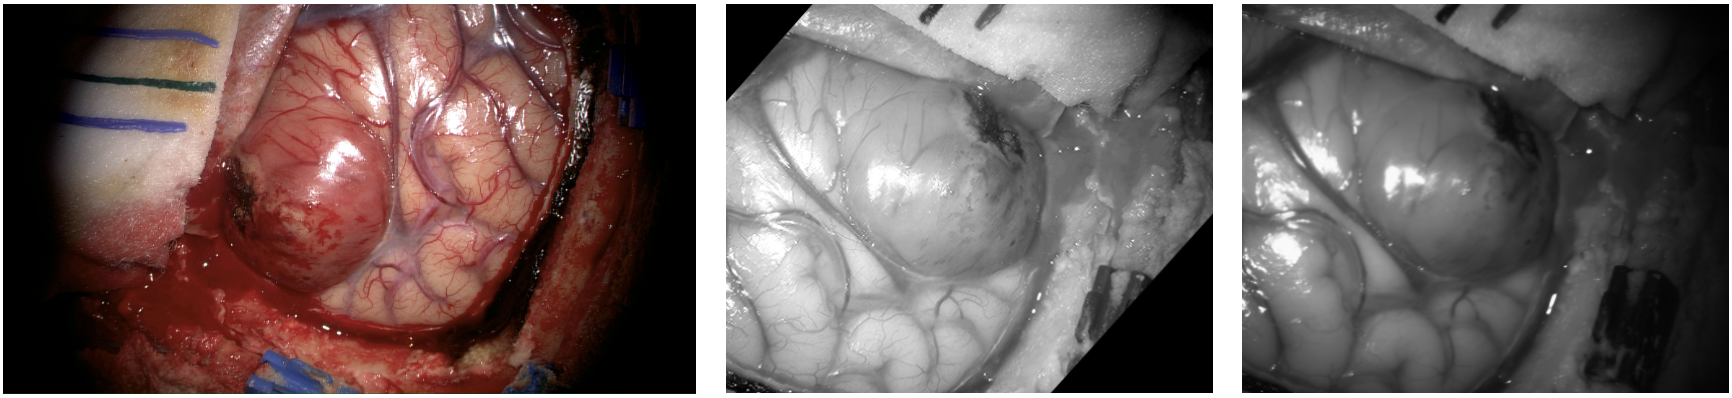
\includegraphics[width=\textwidth]{figures/global-reg.png}
    \caption{A microscope image (left), the registered microscope image (middle) and the reference spectral image (right).}
    \label{fig:global-reg}
\end{minipage}
\end{figure}

\paragraph{}
Figure \ref{fig:global-reg} illustrates the result of global registration. We can see an \acrshort{rgb} microscope image on the left-hand side of the figure. In the middle, we can see the green channel of the microscope image aligned into the same perspective as the reference spectral image on the right. Therefore, the figure shows that we can register microscope images with the spectral image stacks.

\subsection{Finer Registration}
\paragraph{}
Similar to the global registration, the finer registration was also evaluated by comparing the channels of each image. The results for the finer registration are as follows

\begin{center}
\begin{table}[h]
\centering
\begin{tabular}{ c c c c c c c } 
 & \multicolumn{2}{c}{GMSD\^{}} & \multicolumn{2}{c}{SSIM*} & \multicolumn{2}{c}{PSNR*} \\
\hline
Channel & Before & After & Before & After & Before & After \\
\hline
Red              & .153          & \textbf{.146} & .417          & \textbf{.474} & 7.993           & \textbf{8.444} \\
Green            & .159          & \textbf{.154} & .340          & \textbf{.368} & 12.322          & \textbf{12.437} \\
Blue             & \textbf{.164} & .168          & \textbf{.141} & .130          & \textbf{12.544} & 12.502 \\
\textbf{Average} & .159          & \textbf{.156} & .293          & \textbf{.324} & 10.953          & \textbf{11.128} \\
\hline
\end{tabular}

\vspace{0.2cm}
\^{} lower is better --- * higher is better

\caption{Similarity metrics for finer registration.}
\label{table:finer-reg}
\end{table}
\end{center}

\paragraph{}
Table \ref{table:finer-reg} shows some interesting results of the finer registration. On average, the similarity metric values are better after finer registration has been done. The same can also be said for the red and green channels. However, the table shows that the image is more similar for the blue channel before doing the finer registration. Therefore, the finer registration process helps align the microscope images and spectral image stacks.

\paragraph{}
Visualisation between images without and with finer registration can be seen through the video linked in appendix \ref{appendix:finer-reg-res}. The video shows the difference by switching between a registered microscope image and the two images looped several times. If we look closely at the video, we can see that some regions of the image do not align with the microscope image in the image without finer registration on the left. On the other hand, in the image with finer registration on the right, there is only minimal structural change between it and the registered microscope image. The video shows a finer registration process is needed to align the microscope and spectral images further.

\subsection{Pipeline}
\paragraph{}
Now that we have shown that we can align the microscope images and the spectral image stack, we can use the overall transformation to align the labels. Examples of pairs of spectral images and their corresponding labels can be seen in figure \ref{fig:reg-label}. The tumour core is dark-coloured, as shown in the label images on the right and aligned to their position on the spectral images on the left.

\begin{figure}[h]
\centering
\begin{minipage}[h]{\textwidth}
    \centering
    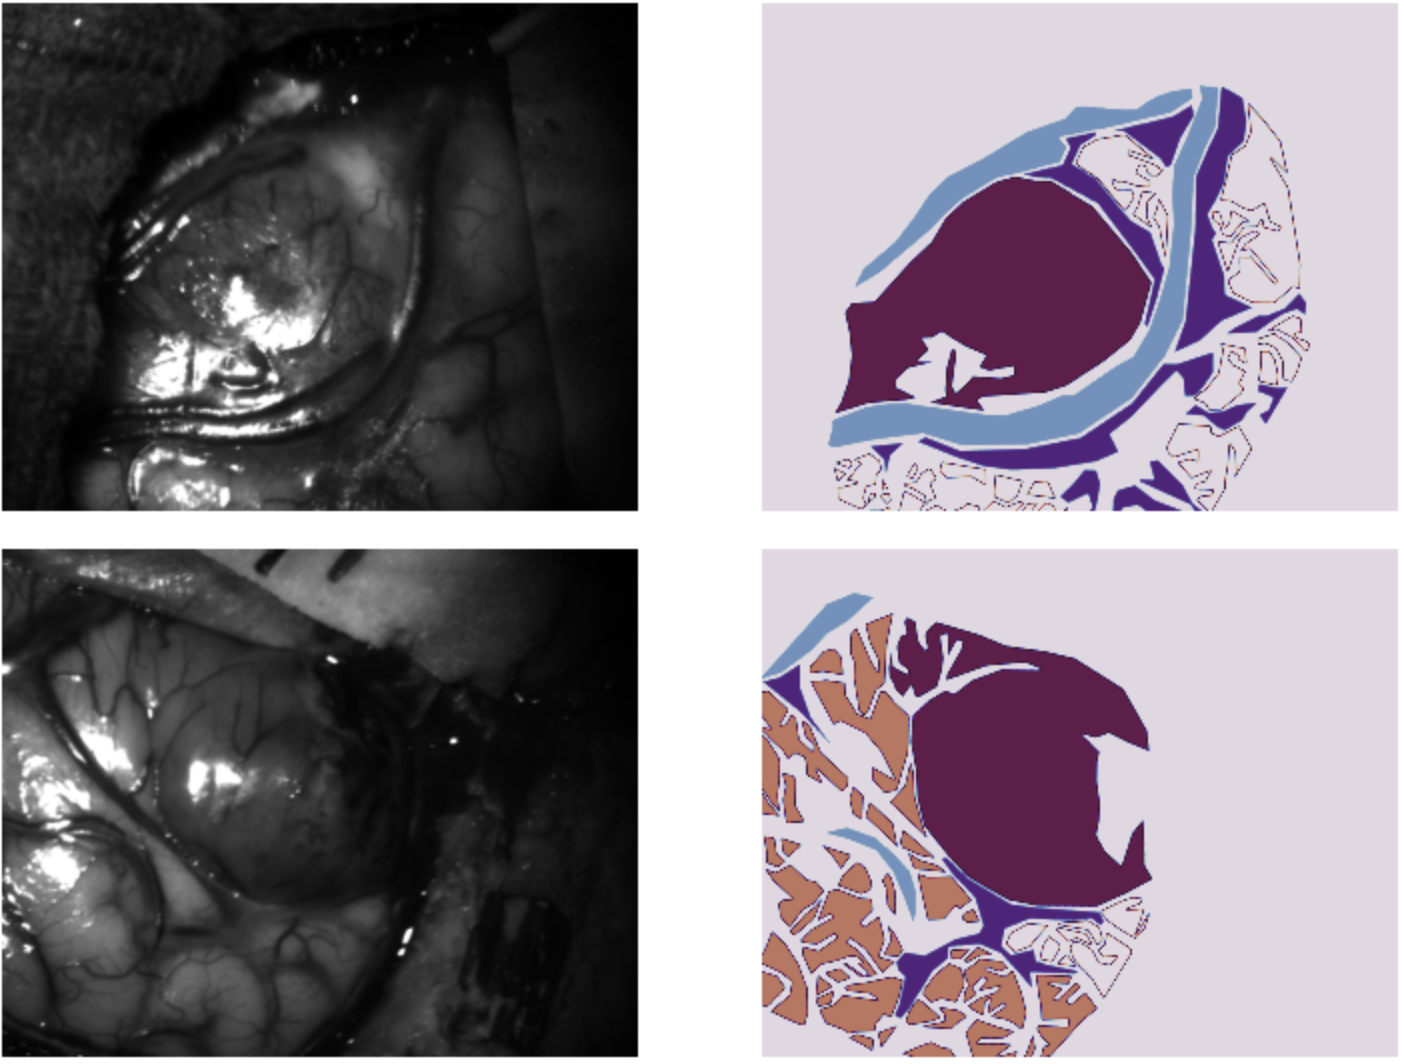
\includegraphics[width=\textwidth]{figures/reg-label.png}
    \caption{Spectral images (left column) and their corresponding labels (right column).}
    \label{fig:reg-label}
\end{minipage}
\end{figure}


\section{Image Analysis}
\paragraph{}
This section will discuss using registered spectral image stack and labels to classify tumour tissue. Evaluations based on similarity metrics and visual assessment were used to compare the results between learning models similar to the registration pipeline. However, in this case, we used different similarity metrics that fit the classification problem. The similarity metrics that were used were intersection over union (\acrshort{iou}), Dice coefficient \cite{dice_measures_1945} and the area under the receiver operator characteristic (\acrshort{roc}) curve (\acrshort{auc}).

\paragraph{}
The \acrshort{iou} is a ratio between the intersection and the total area between two regions. For binary classification, the \acrshort{iou} can be calculated as a function of true positives (TP), true negatives (TN), false positives (FP) and false negatives (FN) as follows

\begin{equation}
    \text{\acrshort{iou}} =
    \frac
        {\text{TP}}
        {\text{TP} + \text{FP} + \text{FN}}
\end{equation}

\paragraph{}
The Dice coefficient is also a ratio of correctly categorised regions. However, unlike \acrshort{iou}, it emphasises true positive regions by doubling the regions' values. The Dice coefficient can be calculated as

\begin{equation}
    \text{DICE} =
    \frac
        {2 \text{TP}}
        {2 \text{TP} + \text{FP} + \text{FN}}
\end{equation}

\paragraph{}
The \acrshort{auc} is the area under the curve bounded by the \acrshort{roc} line. The \acrshort{roc} line is defined by a set of data points with the false positive rate (FPR) as its x-axis and the true positive rate (TPR) as its y-axis. Using TP, TN, FP and FN, we can define FPR and TPR as

\begin{equation}
    \text{FPR} =
    \frac{\text{FP}}{\text{FP} + \text{TN}}
\end{equation}

\begin{equation}
    \text{TPR} =
    \frac{\text{TP}}{\text{TP} + \text{FN}}
\end{equation}

\begin{center}
\begin{table}[h]
\centering
\begin{tabular}{ c c c c c } 
 & \multicolumn{2}{c}{XGBoost} & \multicolumn{2}{c}{U-Net} \\
\hline
Metrics & W/O & W/ & W/O & W/ \\
\hline
IoU  & 0.132 & \textbf{0.176} & 0.701 & \textbf{0.863} \\
Dice & 0.188 & \textbf{0.197} & 0.832 & \textbf{0.853} \\
AUC  & 0.624 & \textbf{0.645} & 0.651 & \textbf{0.724} \\
\hline
\end{tabular}

\vspace{0.2cm}
W/: with finer registration --- W/O: without finer registration

\caption{Metrics of image analysis.}
\label{table:finer-reg}
\end{table}
\end{center}

\paragraph{}
In table \ref{table:finer-reg}, we can see that the result is better for all metrics and classification methods using images that went through finer registration. Furthermore, based on the similarity metric scores, U-Net performs better classification than XGBoost.

\begin{figure}[h]
\centering
\begin{minipage}[h]{\textwidth}
    \centering
    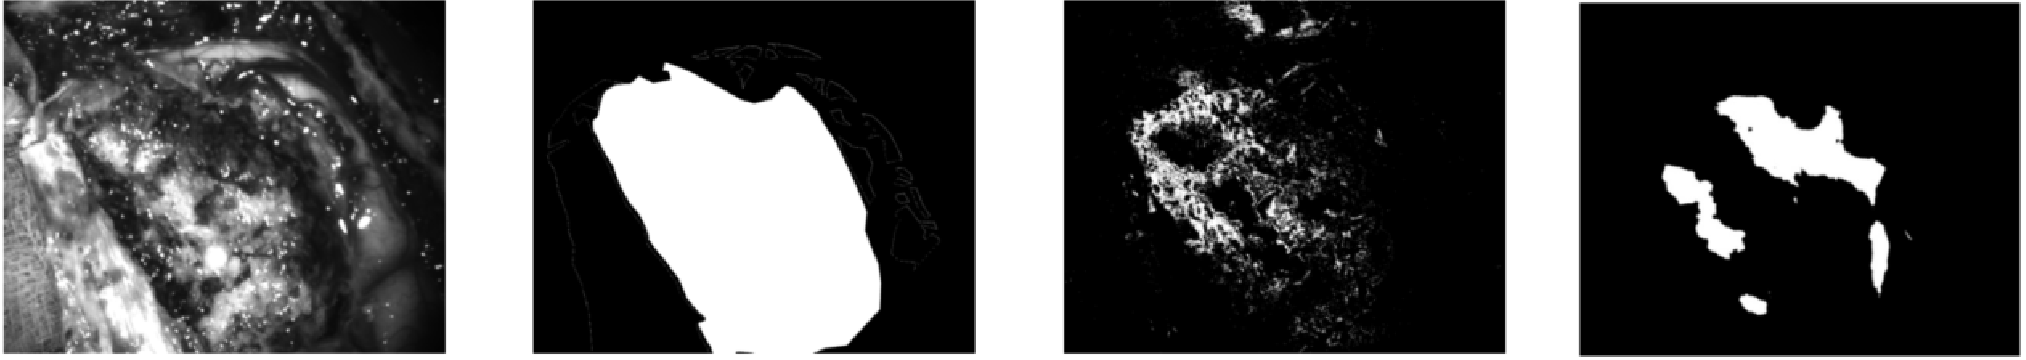
\includegraphics[width=\textwidth]{figures/analysis.png}
    \caption{From left to right: a spectral image, label image corresponding to the spectral image, the image label classified using XGBoost and the image label classified using U-Net.}
    \label{fig:analysis}
\end{minipage}
\end{figure}

\paragraph{}
The classification result can be seen on the two right-most images in figure \ref{fig:analysis}. While the similarity metrics are promising, visual assessment of the label prediction images suggests that both models still need improvement. In the label image predicted using XGBoost, the label can only be seen as specks or noncontiguous regions. As for the label image predicted using U-Net, the label is predicted correctly but only in small regions of the image. Therefore, further analysis will be needed to utilise the acquired multi-spectral image dataset fully.


%%%%%%%%%%%%%%%%%%%%%%%%%%%%%%%%%%%%
\chapter{Conclusion and Future Works}

\paragraph{}
In summary, this project shows that the acquired is useful and can be used for further analysis. While the labels do not match the spectral images, a pipeline of registration techniques solves the problem by aligning the images. Preliminary analysis and literature review revealed that classification based on spectral image stack can be done, but further work remains to be seen on the type of learning model suitable for the dataset.

\section{Future Works}
\paragraph{}
There are only several tissue labels present in the dataset. The type and number of labels that would be needed for the tumour classification problem still need to be determined. Moreover, the full surgical environment analysis will require more labels for other tissue types and surgical instruments. However, as the number of label types increases, the problem may become more complex and harder to solve.

\paragraph{}
A limited number of image similarity metrics are available for different image modalities. While metrics such as \acrshort{gmsd} and \acrshort{ssim} help determine a change in similarity, the resulting value would still vary when comparing multimodal images. This makes it quite challenging to objectively evaluate the similarity between the microscope image and the spectral image stack from the dataset. A feature extraction and correspondence method based on a neural network architecture may solve this problem in the future.

\paragraph{}
Lastly, as shown in the preliminary analysis, learning models based on deep neural networks may perform better than classical machine learning models. It might also be beneficial to try methods from domains outside medicine that use \acrshort{msi}, such as geosensing.


%%%%%%%%%%%%%%%%%%%%%%%%%%%%%%%%%%%%
%% bibliography
\renewcommand{\bibname}{References}
% \bibliographystyle{ieeetr}
\bibliographystyle{unsrtnat}
\bibliography{ref}


%%%%%%%%%%%%%%%%%%%%%%%%%%%%%%%%%%%%
%% appendix
\appendix

\chapter{Videos}

\section{Tissue Displacement}
\label{appendix:tissue-disp}
\url{https://youtu.be/1u3UvhZq-hI}

\section{Stack Registration Result}
\label{appendix:stack-reg-res}
\url{https://youtu.be/afG8nFMP9TY}

\section{Finer Registration Result}
\label{appendix:finer-reg-res}
\url{https://youtu.be/pH_cC5lDyPM}


%%%%%%%%%%%%%%%%%%%%%%%%%%%%%%%%%%%%
\end{document}
